% -------------------------------------------------

\chapter{Examples} %2 - the elastic Marmousi2 model}
% \label{The Marmousi2 model}

% -------------------------------------------------

% % -------------------------------------------------
% 
% \chapter{Example 3 - inversion of ultrasonic data}
% \label{Example 3}
% 
% % -------------------------------------------------
% 
% \section{Homogenous plexiglas bloc model}
% The second example consists of real data which was recorded at a Plexiglas bloc with size of 10*15*20 cm. Using a simple regression a Rayleigh-wave-velocity of 1277.2 m/s could be estimated. A waveform inversion with DENISE can be achieved in XX steps. The necessary MATLAB scripts are located in the \textit{/mfiles/US} directory.    
% 
% \begin{figure}[bh]
% \includegraphics[width=15cm]{figures/ultrasonic/Plexiglasblock.jpg}
% \caption{Photo of the homogenous plexiglas bloc with ultrasonic acquisition geometry.}
% \label{Plexiglasblock.jpg}
% \end{figure}
% 
% \clearpage
% 
% \begin{enumerate}
% \item First we have to find some initial guess for the elastic parameters of plexiglas. The parameters in \cite{zerwer:2000} seem to be in good agreement with the measured Rayleigh wave velocity: $\rm{Vp=2700\; m/s}$, $\rm{Vs=1370\; m/s}$ and $\rm{\rho=1190\; kg/m^3}$ leads to a Rayleigh wave velocity of $\rm{VR=1280\; m/s}$. Assuming a maximum frequency $\rm{f_{max} = 600\; kHz}$ and using the grid disperson-, Courant criterion and the extension of the acquisition geometry the following FD-model parameters are required:
% \begin{itemize}
% \item DH = 2.0e-4 m
% \item DT = 5.2e-8 s
% \item NX = 860 gridpoints, NY = 200 gridpoints
% \item NT = 3077 time steps
% \end{itemize}
% The necessary files for the input parameters DENISE\_US.inp, source\_ricker.dat, source\_spike.dat and source\_wavelet.dat, receiver\_US.dat and model definition half\_space.c are located in the directory DENISE/genmod/US. Copy these files to the DENISE/par and DENISE/src directories, respectively. Set 
% {\color{blue}{\begin{verbatim}
% QUELLART=1
% SOURCE_FILE = ./source/source_ricker.dat
% SNAP=3
% INVMAT=10
% \end{verbatim}}}
% in the parameter file \textit{DENISE$\_$US.inp} and start a first test model run:
% {\color{blue}{\begin{verbatim}
% -bash-2.05b$:~/DENISE/par> mpirun -np 4 ../bin/denise DENISE_US.inp 
% \end{verbatim}}}
% Merge the resulting wavefield snapshots with 
% {\color{blue}{\begin{verbatim}
% -bash-2.05b$:~/DENISE/par> snapmerge ../bin/denise < DENISE_US.inp 
% \end{verbatim}}}
% Copy the file snap/waveform\_forward.bin.rot to the snap-directory in mfiles/US. With the MATLAB-script US\_snap you can visualize the propagation of the surface wave. The script is self-explanatory. Set 
% {\color{blue}{\begin{verbatim}
% 14 % name of the snap file
% 15 file_div='snap/waveform_forward.bin.rot';
% [...]
% 20 % optimize clipping values
% 21 caxis_value_vp1=-5e-1;
% 22 caxis_value_vp2=5e-1;
% [...]
% 24 % define first and last frame to display
% 25 firstframe=1;
% 26 lastframe=50;
% [...]
% 28 % gridsize and grid spacing (as specified in parameter-file) 
% 29 NX1glob=1; NX2glob=860;
% 30 NY1glob=1; NY2glob=200; 
% 31 IDX=1; IDY=1;
% 32 dh_glob=2e-4;
% [...]
% 34 % time increment for snapshots:
% 35 TSNAPINC=3e-6; TSNAP1=3e-6;
% \end{verbatim}}}
% and run the script. A few representive snapshots of the Rayleighwave propagation are shown in \FIG{Rayleighwave-propagation}
% \begin{figure}[bh]
% \includegraphics[width=8.5cm]{figures/ultrasonic/US_snap_6.pdf}\includegraphics[width=8.5cm]{figures/ultrasonic/US_snap_10.pdf}\\
% \includegraphics[width=8.5cm]{figures/ultrasonic/US_snap_18.pdf}\includegraphics[width=8.5cm]{figures/ultrasonic/US_snap_27.pdf}\\
% \includegraphics[width=8.5cm]{figures/ultrasonic/US_snap_36.pdf}\includegraphics[width=8.5cm]{figures/ultrasonic/US_snap_44.pdf}\\
% \caption{A few snapshots of the Rayleighwave propagating through the homogenous Plexiglas block.}
% \label{Rayleighwave-propagation}
% \end{figure} 
% \clearpage 
% \item In the next step we take a look at the raw data and convert the ASCII data to SU format. Open the MATLAB-script ASCII2SU.m. Define the location of the plexiglas data:
% {\color{blue}{\begin{verbatim}
% 83 file_name = ['plexiglas_profil_data/',int2str(i),'mm.txt'];
% \end{verbatim}}}
% Each trace of the ultrasonic data is located in a file $\bf{<offset>mm.txt}$, the acquistion geometry is defined in $\bf{readme.txt}$. The range of the offset values, the increment and the sample interval:
% {\color{blue}{\begin{verbatim}
% 63 ntr1=62;          % minimum offset
% 64 ntr2=162;         % maximum offset
% 65 dntr1=10;         % offset interval
% ...
% 69 DT=1.0e-7;        % sampling interval of the US data
% \end{verbatim}}}
% Activate the interpolation of the data and define the sampling interval and number of time steps in DENISE:
% {\color{blue}{\begin{verbatim}
% 41 INTERP=1;
% 42 DT1=5.2e-8;     % sampling rate for DENISE
% 43 nt_DENISE=3462; % number of time steps in DENISE
% \end{verbatim}}}
% Define a time delay, which makes the later source wavelet inversion much easier: 
% {\color{blue}{\begin{verbatim}
% 23 DELAY=1;
% 24 delay=2.8e-5;   % time delay for real data
% \end{verbatim}}}
% and finally activate the output of the SU file and enter a name for the SU file:
% {\color{blue}{\begin{verbatim}
% 55 WRITE=1;
% 56 % name of output SU file
% 57 imfile=['plexiglas_profil_data/DENISE_plexiglas_y.su.shot1'];
% \end{verbatim}}}
% After running the script you get the following seismic section: 
% \begin{figure}[bh]
% \centering
% \includegraphics[width=15cm]{figures/ultrasonic/plexiglas_step1.png}
% \caption{Elastic waveform inversion of ultrasonic data - step 1 (raw data).}
% \label{Plexiglas_step_1}
% \end{figure}
% \clearpage
% \item The data looks a bit noisy, therefore activate the bandpass frequency filter, where f1, f2, f3 and f4 define the corner frequencies:
% {\color{blue}{\begin{verbatim}
% 47 FILTER=1;
% 48 f1=35000;
% 49 f2=40000;
% 50 f3=450000;
% 51 f4=500000;
% \end{verbatim}}}
% We want to restrict the inversion to the wavelet of the first arrival. Therefore activate the time window:
% {\color{blue}{\begin{verbatim}
% 28 TWIN=1;
% 29 twinc=5.36e-5+delay; % center of time window
% 30 twinp=1e-5;          % twinc + twinp
% 31 twinm=1e-5;          % twinc - twinm
% 32 ad=1e12;             % damping parameter
% 33 vnmo=1280;           % velocity of the Rayleigh wave
% \end{verbatim}}}
% The parameter twinc should be approximately at the center of the first arrival wavelet. twinp and twinm define the length of the time window, ad the damping parameter and vnmo the normal moveout of the Rayleigh wave. Optimize these parameters until the window is well defined. For each trace the value of twinc will be written to 
% {\color{blue}{\begin{verbatim}
% 278 imfile=['picks_1.dat'];
% \end{verbatim}}}
% An optimized seismic section is shown in \FIG{Plexiglas_step_2}. The yellow dots denote the time twinc, the blue dots the time twinc+twinp and the red dots the time twinc-twinp, respectively.   
% \begin{figure}[bh]
% \centering
% \includegraphics[width=15cm]{figures/ultrasonic/plexiglas_step2.png}
% \caption{Elastic waveform inversion of ultrasonic data - step 2 (optimized seismic section with time window).}
% \label{Plexiglas_step_2}
% \end{figure}
% \clearpage
% \item Copy the generated SU-file \textit{DENISE$\rm{\_}$plexiglas$\rm{\_}$y.su.shot1} to the data directory \textit{DENISE/par/su/plexiglas} and the file with the definition of the time window \textit{picks$\_$1.dat} to \textit{DENISE/par/picked$\_$times}.
% \item Define 
% {\color{blue}{\begin{verbatim}
% QUELLART=6
% SOURCE_FILE = ./source/source_spike.dat
% SNAP=0
% INVMAT=10
% TWIN=0
% INV_STF=0
% \end{verbatim}}}
% in the parameter file \textit{DENISE$\_$US.inp}, set the time delay td in the source-file \textit{source$\_$spike.dat} to 0.0 s and run a forward model.   
% \item Copy su/DENISE\_US\_y.su.shot1.it1 to the FD\_seis directory and open the Matlab script Plot\_US\_Residuals.m. Be sure that the parameters delay, twinc, twinp, twinm, ad, vnmo, f1, f2, f3, f4, ntr, ntr1, ntr2, dntr1, DT1 and in\_data are equal to the definitions in ASCII2SU.m. Turn the time window off (TWIN=0). After running the script you should get the following seismic sections. On the left side a comparison of the seismic section between the model data (red) and the field data (black) and on the right the data residuals:
% \begin{figure}[bh]
% \centering
% \includegraphics[width=18cm]{figures/ultrasonic/plexiglas_step5.png}
% \caption{Elastic waveform inversion of ultrasonic data - step 5 (first model result).}
% \label{Plexiglas_step_5}
% \end{figure}
% \clearpage
% \item Zoom into the first trace of the data comparison and pick time values of the measured t1 and modelled wavelets t2, respectively (\FIG{Plexiglas_step_6}). From this values calculate the time delay td between the wavelets. 
% In this example, t1=8.05e-5 s, t2=4.93e-5 s and td=t1-t2=3.12e-5 s.  
% \begin{figure}[bh]
% \centering
% \includegraphics[width=16cm]{figures/ultrasonic/plexiglas_step6.pdf}
% \caption{Elastic waveform inversion of ultrasonic data - step 6 (measure time delay).}
% \label{Plexiglas_step_6}
% \end{figure}
% \clearpage
% \item Change the time delay td in source\_spike.dat to the measured value, run a new model, copy the resulting DENISE\_US\_y.su.shot1.it1 file to the FD\_seis directory again and check if there is still a significant time delay present. Optimize it further until the wavelets approximately fit (\FIG{Plexiglas_step_7}).   
% \begin{figure}[bh]
% \centering
% \includegraphics[width=16cm]{figures/ultrasonic/plexiglas_step7.pdf}
% \caption{Elastic waveform inversion of ultrasonic data - step 7 (optimum wavelet fit).}
% \label{Plexiglas_step_7}
% \end{figure}
% \item After fitting the arrival times of the wavelets approximately we proceed with the source wavelet inversion. Copy the initial source wavelet from start/half\_space\_source\_signal.0.su.shot1 to US/wavelet. Open the matlab script est\_source\_wavelet.m and check if the parameters delay, twinc, twinp, twinm, ad, vnmo, f1, f2, f3, f4, ntr, ntr1, ntr2, dntr1, DT1, in\_data and in\_model are consistent with those in the other two matlab scripts and additionally define in\_source. Set the Marquardt-Levenber damping factor epsilon=0.0 and run the script. With no regularization the data fit looks nearly perfect (\FIG{Plexiglas_step_8a}), but the resulting source wavelet looks very unrealistic and contains a lot of spikes. When increasing the damping factor epsilon (f.e. to epsilon=1e1) the solutions are damped and become more plausible, while the data misfit increases (\FIG{Plexiglas_step_8b}). Optimize epsilon until you find a good compromise between plausible source wavelet and minimum data misfit. 
% \begin{figure}[bh]
% \centering
% \includegraphics[width=16cm]{figures/ultrasonic/plexiglas_data_step8_lam_0.pdf}
% \includegraphics[width=16cm]{figures/ultrasonic/plexiglas_wavelet_step8_lam_0.pdf}
% \caption{Elastic waveform inversion of ultrasonic data - step 8. Resulting seismic sections for the estimated source wavelet (top) with no regularization ($\epsilon=0.0$) and the estimated source wavelet (bottom).}
% \label{Plexiglas_step_8a}
% \end{figure}
% \clearpage
% \begin{figure}[bh]
% \centering
% \includegraphics[width=16cm]{figures/ultrasonic/plexiglas_data_step8_lam_1e1.pdf}
% \includegraphics[width=16cm]{figures/ultrasonic/plexiglas_wavelet_step8_lam_1e1.pdf}
% \caption{Elastic waveform inversion of ultrasonic data - step 8. Resulting seismic sections for the estimated source wavelet (top) with regularization ($\epsilon=1e1$) and the estimated source wavelet (bottom).}
% \label{Plexiglas_step_8b}
% \end{figure}
% \clearpage
% \item Copy wavelet\_US\_opt.dat to /par/wavelet, edit DENISE\_US.inp
% {\color{blue}{\begin{verbatim}
% SOURCE_FILE = ./source/source_wavelet.dat
% QUELLART = 3
% SIGNAL_FILE = ./wavelet/wavelet_US_opt.dat 
% \end{verbatim}}}
% set the time delay td in the source-file \textit{source$\_$wavelet.dat} to 0.0 and run DENISE again.
% \item Copy DENISE/su/DENISE\_US\_y.su.shot1.it1 to the FD\_seis directory and run the Matlab script Plot\_US\_Residuals.m. You should get the following seismic sections:
% \begin{figure}[bh]
% \centering
% \includegraphics[width=16cm]{figures/ultrasonic/plexiglas_step9.pdf}
% \caption{Elastic waveform inversion of ultrasonic data - step 9 (model result with estimated source wavelet).}
% \label{Plexiglas_step_9}
% \end{figure}
% \clearpage
% \item Similar to step 6 measure the time delay td in Matlab. In this case the first arrival of the measured data is earlier than the modelled arrival. Therefore the time delay is negative, td=-5.875e-5 s:
% \begin{figure}[bh]
% \centering
% \includegraphics[width=16cm]{figures/ultrasonic/plexiglas_step10.pdf}
% \caption{Elastic waveform inversion of ultrasonic data - step 10 (measure time delay).}
% \label{Plexiglas_step_10}
% \end{figure}
% \clearpage
% \item Change the time delay td in source\_wavelet.dat according to the measured time delay and run DENISE again. Copy the resulting DENISE/su/DENISE\_US\_y.su.shot1.it1 to the FD\_seis directory and run the Matlab script Plot\_US\_Residuals.m. You should get the following seismic sections with an approximately well fitted first arrival wavelet:
% \begin{figure}[bh]
% \centering
% \includegraphics[width=16cm]{figures/ultrasonic/plexiglas_step11.pdf}
% \caption{Elastic waveform inversion of ultrasonic data - step 11 (model result with estimated source wavelet and corrected time delay).}
% \label{Plexiglas_step_11}
% \end{figure}
% 
% \end{enumerate}

% \chapter{Example 4 - shallow seismics}
% \label{example4}

\section{Toy Example Shallow Seismics: Inversion of Viscoelastic Observations}
You can find the input files for the small toy example in the directory \texttt{par/in\_and\_out/toy\_example}. To run the example you can use the shell script \texttt{run\_toy\_example.sh} in the directory \texttt{par}. It is adjusted for a PC with at least 4 CPUs. If you have less CPUs you have to adjust the number of processors in the input files as well as in the call of DENISE in the shell script. The shell script includes all relevant steps. First all libraries and DENISE are compiled. (Do not get nervous about the huge output during compiling.) If you run into problems during this step you maybe have to adjust the variables in \texttt{Makefile\_var} in the directory \texttt{contrib}. Afterwards DENISE starts to simulate observed data for the inversion. The simulated seismograms are renamed for the inversion and DENISE is again compiled with another model function which creates the initial models for the inverison on the fly (see section~\ref{gen_of_mod}). The last step in the shell script is the call of DENISE to start the inversion.\\

The true model used for the simulation of the observed data is shown in Figure~\ref{Rheinstetten_true_model} whereat the shot positions are marked by the red stars and the CPML frame is marked by the black dashed line. We consider a viscoelastic medium in this test and approximate a constant quality factor of $Q_s=Q_p=20$ in the analyzed frequency band up to 70\,Hz with three relaxation mechanisms of a generalized standard linear solid. The 36 two component receivers used in the inversion are located equidistantly between the sources with a receiver spacing of 1\,m.\\

In the inversion we only inverted for the shear wave velocity model. The initial model is a linear gradient and is shown in Figure~\ref{Rheinstetten_initial_vs_model}.  For the P wave velocity model as well as for the density model the true models (see Figure~\ref{Rheinstetten_true_model}\subref{true-vp-model-Rheinstetten} and \subref{true-rho-model-Rheinstetten}) are used. Furthermore, we use the correct rheological model.\\

You will need less than 1~GB working memory to run the inversion and approximately 250\,MB of data are written to hard disk. Normally 137~iteration steps are calculated and the inversion will take approximately 6 hours. The inversion results for the shear wave velocity are shown in Figure~\ref{Rheinstetten_inversion_result}. Figure~\ref{Rheinstetten_inversion_result}\subref{inv-vs-model-Rheinstetten} shows an image plot and Figure~\ref{Rheinstetten_inversion_result}\subref{vertical-vel-profiles-Rheinstetten} shows vertical velocity profiles through the shear wave velocity models (thick grey line: true model; black dashed line: initial model; blue line: inverted model at $x=20$\,m; red dashed line: inverted model at $x=25$\,m).\\

You can use the script \texttt{mfiles/Plot\_results\_toy\_example.m} to visualize the results of the toy example. This script can be used with Matlab or Octave.


\begin{figure}[ht]
\centering
\subfloat[][]{%
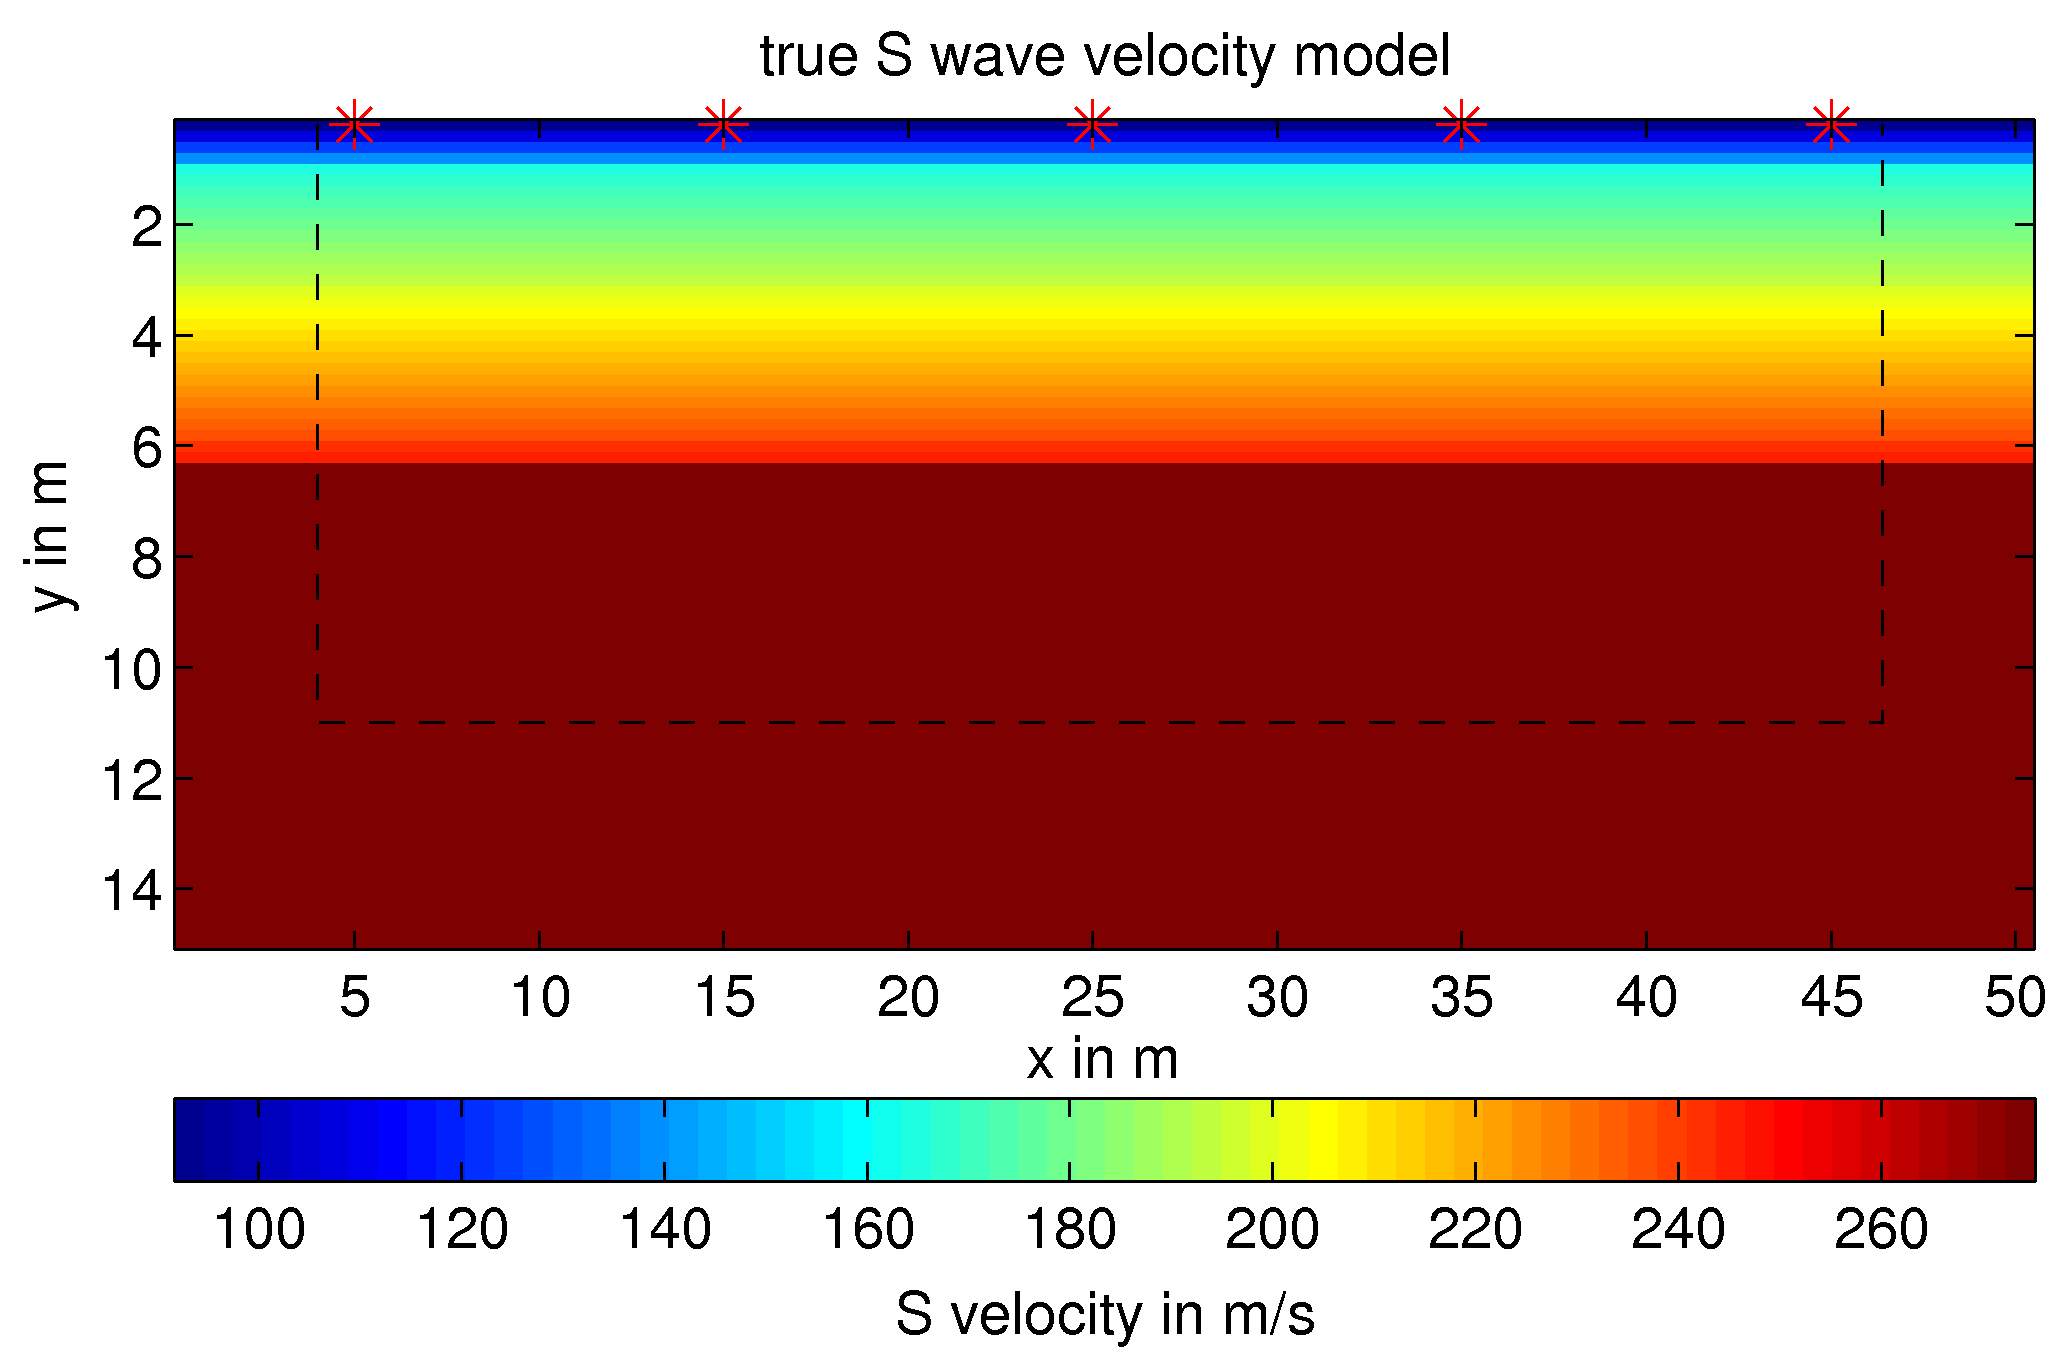
\includegraphics[width=10cm]{figures/Rheinstetten/true_vs_model}%
\label{true-vs-model-Rheinstetten}}\\%
\subfloat[][]{%
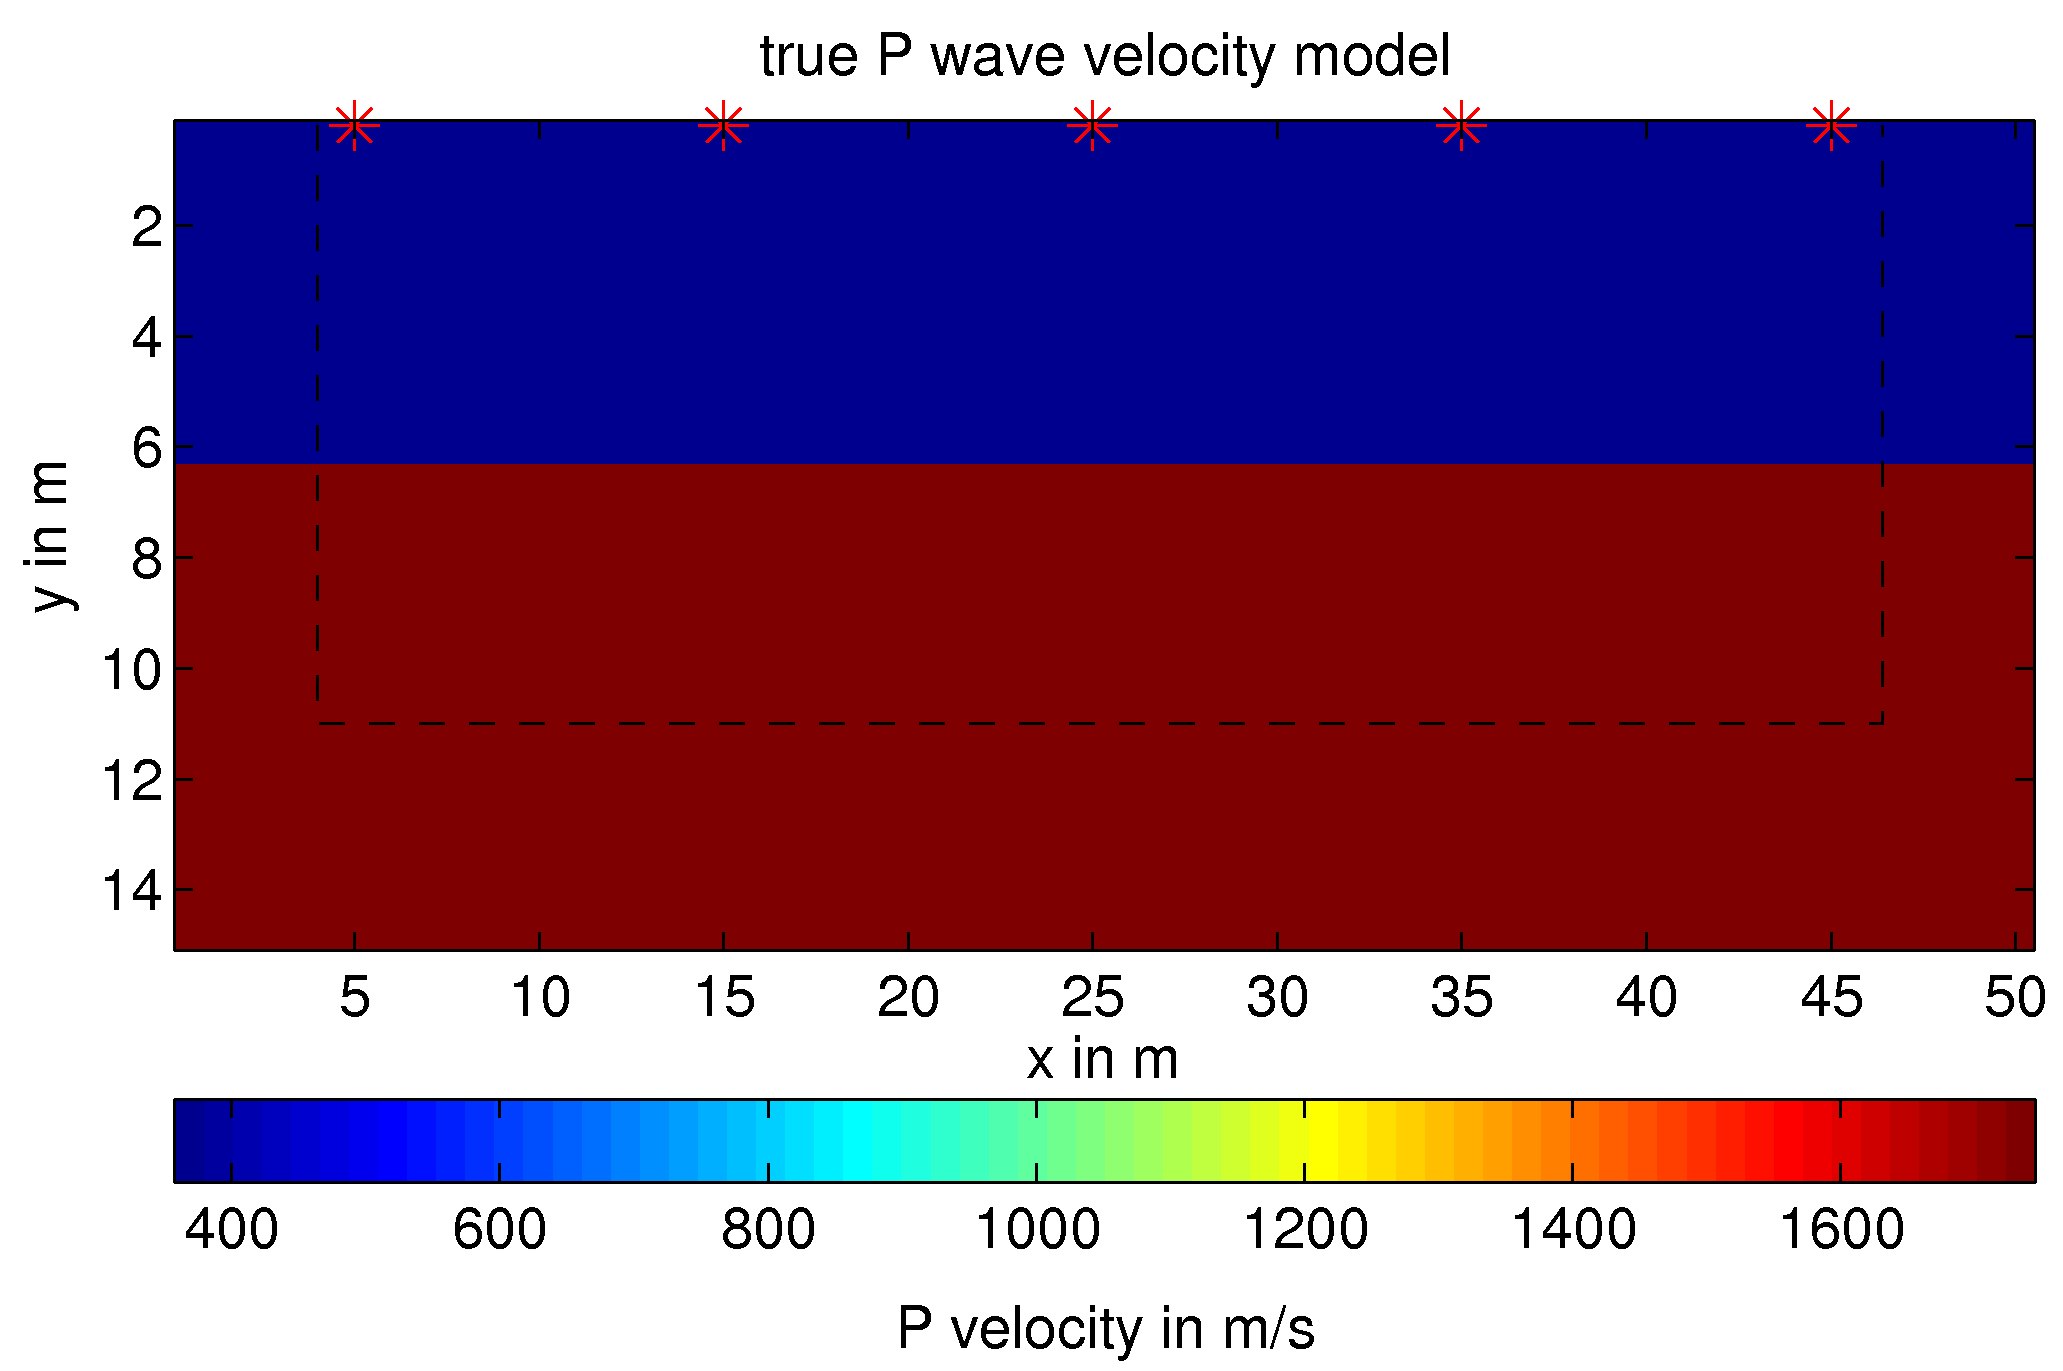
\includegraphics[width=10cm]{figures/Rheinstetten/true_vp_model}%
\label{true-vp-model-Rheinstetten}}\\%
\subfloat[][]{%
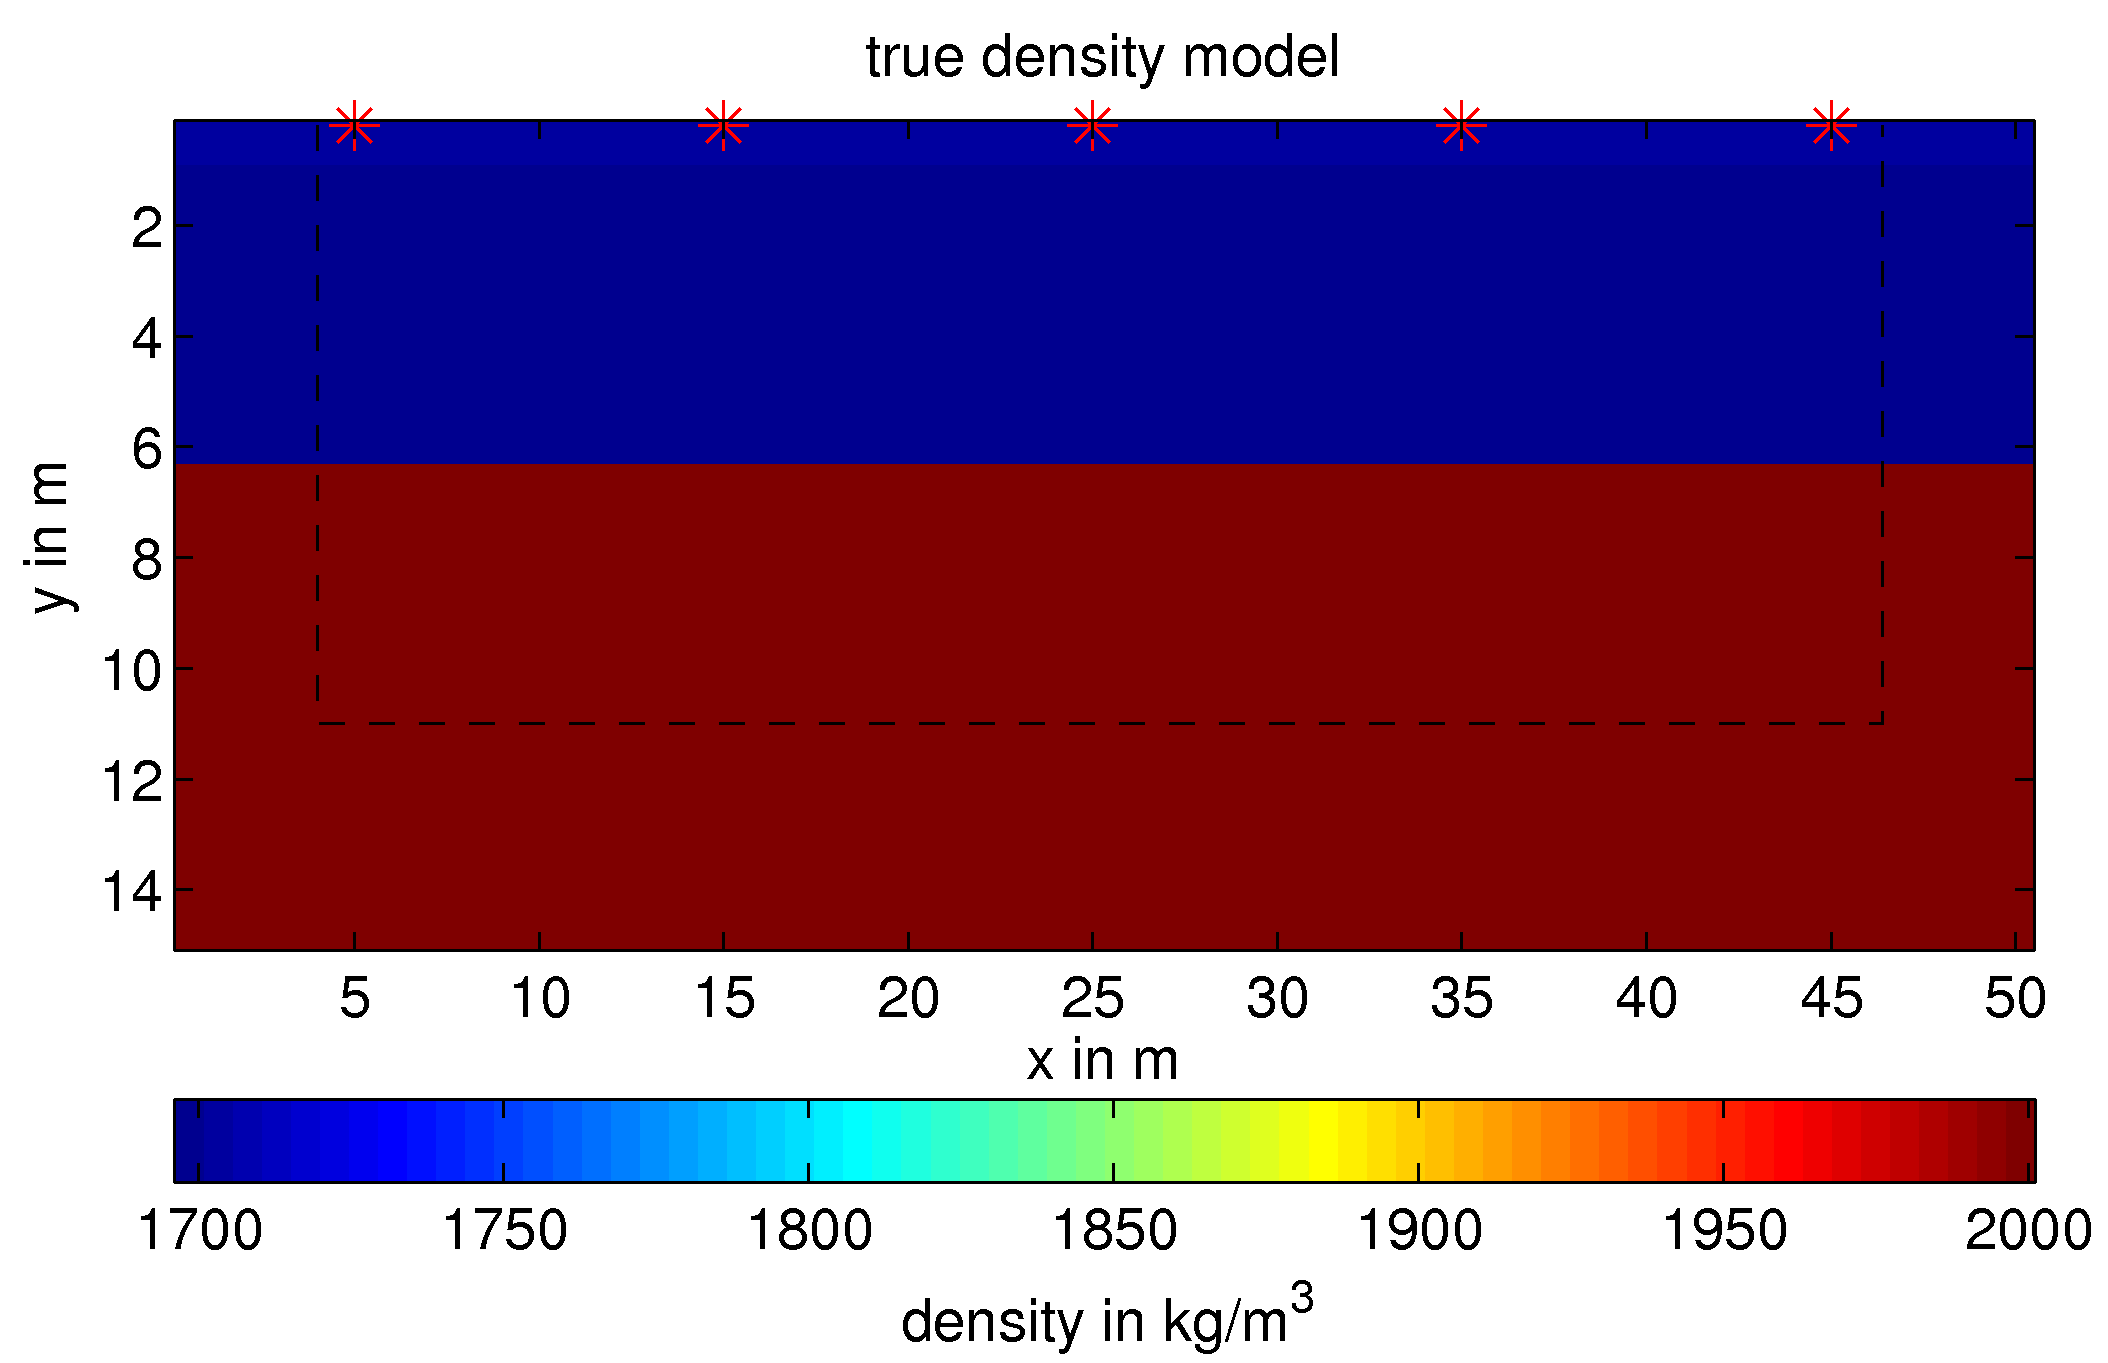
\includegraphics[width=10cm]{figures/Rheinstetten/true_rho_model}%
\label{true-rho-model-Rheinstetten}}
\caption{True models for \protect\subref{true-vs-model-Rheinstetten} the S wave velocity, \protect\subref{true-vp-model-Rheinstetten} the P wave velocity and \protect\subref{true-rho-model-Rheinstetten} the density used for the calculation of observed data. The red stars mark the five shots used in the inversion. The CPML frame is marked by the black dashed line.}
\label{Rheinstetten_true_model}
\end{figure}


\begin{figure}[ht]
\centering
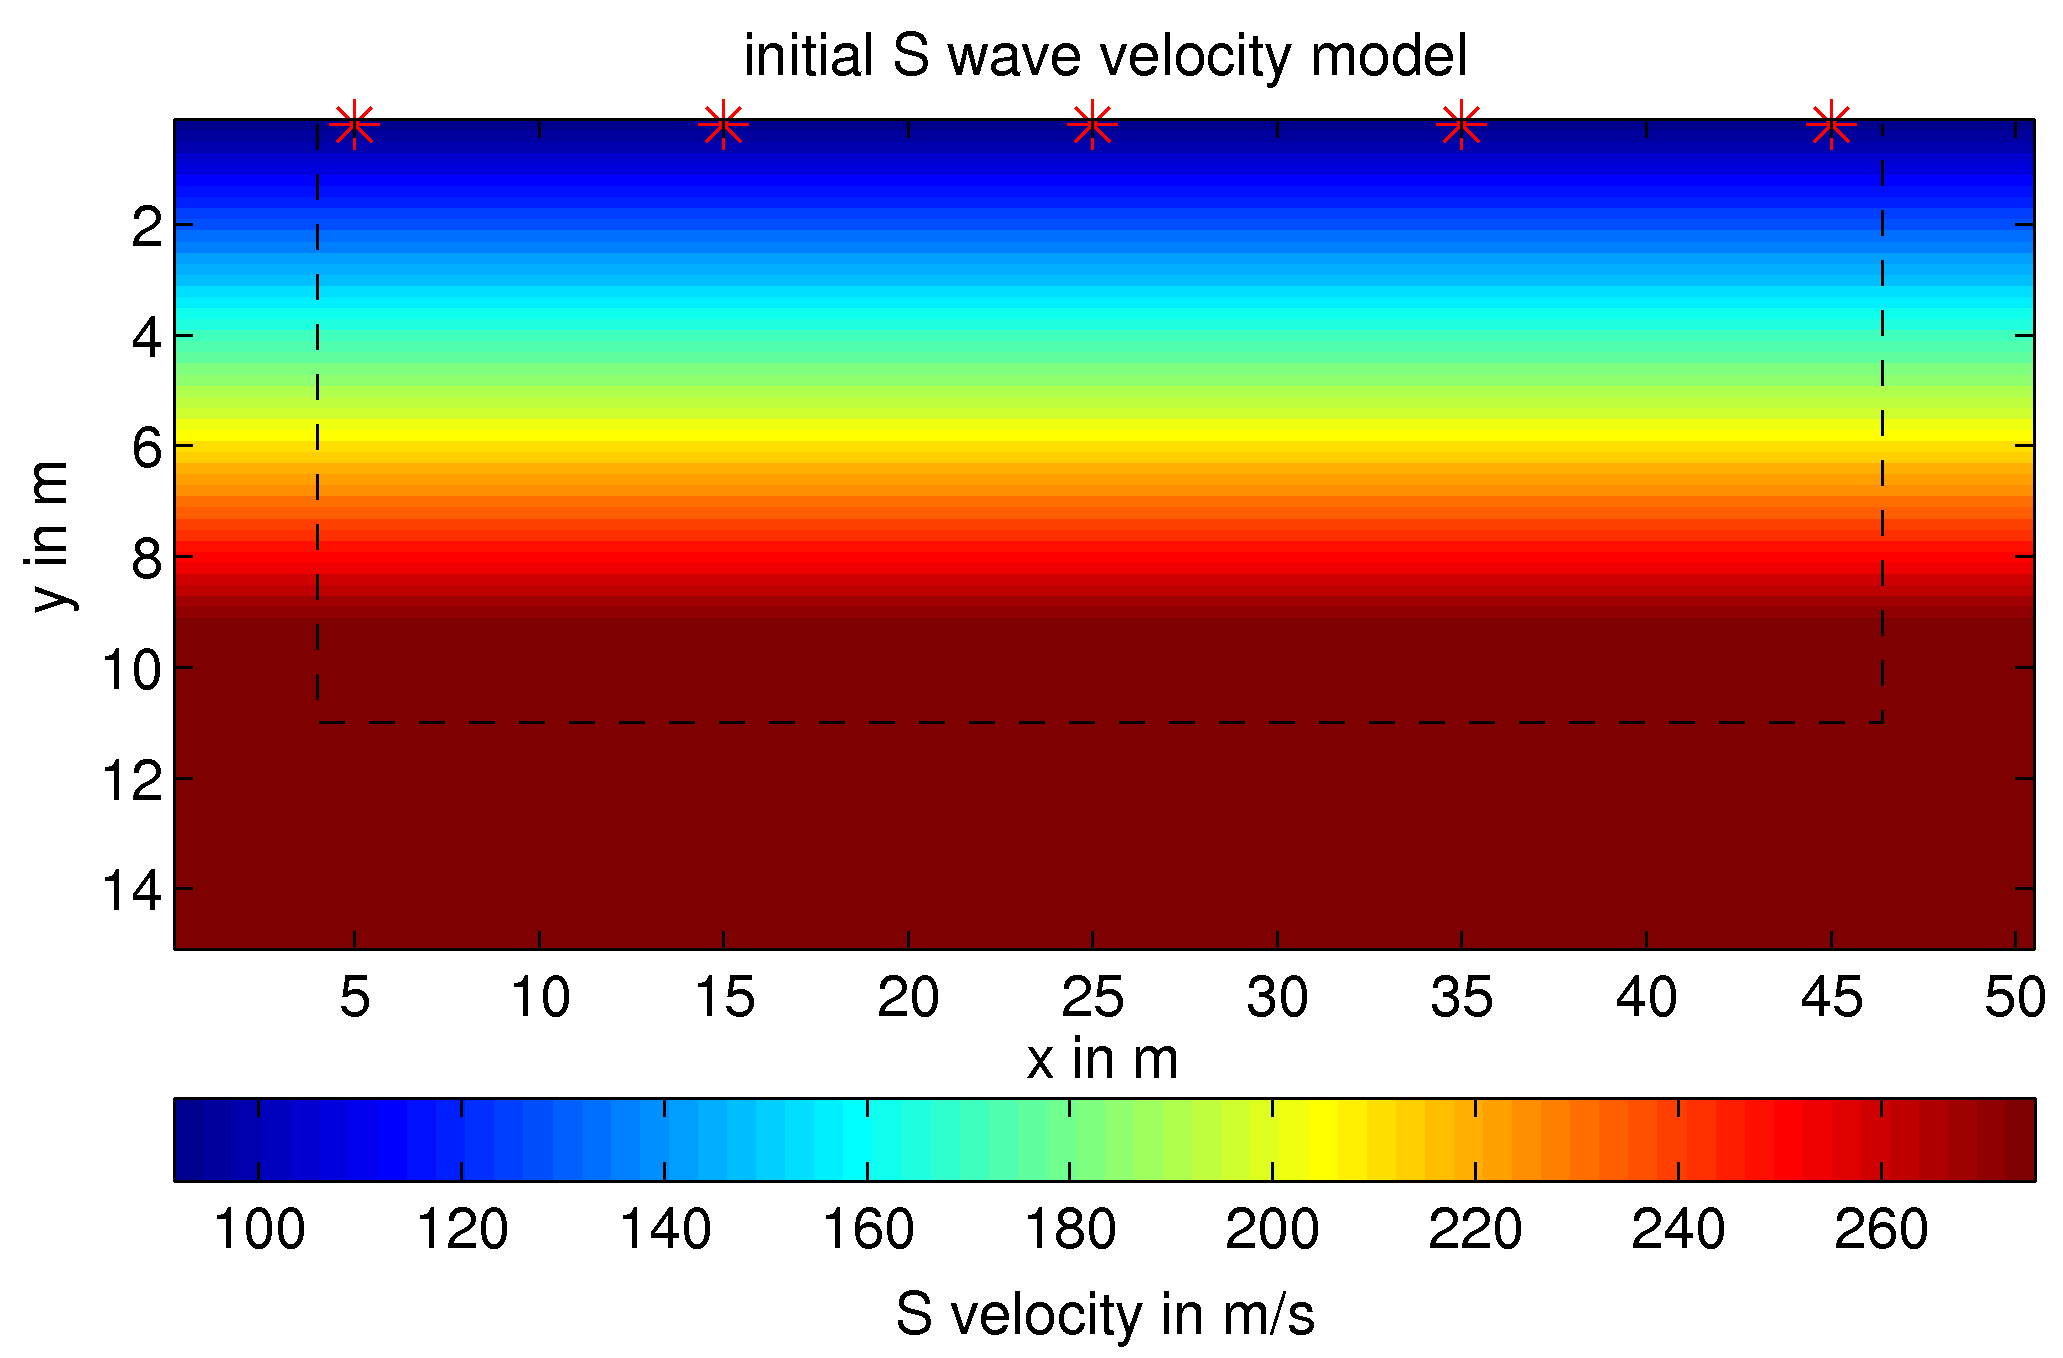
\includegraphics[width=10cm]{figures/Rheinstetten/start_vs_model}
\caption{Initial shear wave velocity model. The red stars mark the five shots used in the inversion. The CPML frame is marked by the black dashed line.}
\label{Rheinstetten_initial_vs_model}
\end{figure}

\begin{figure}[ht]
\centering
\subfloat[][]{%
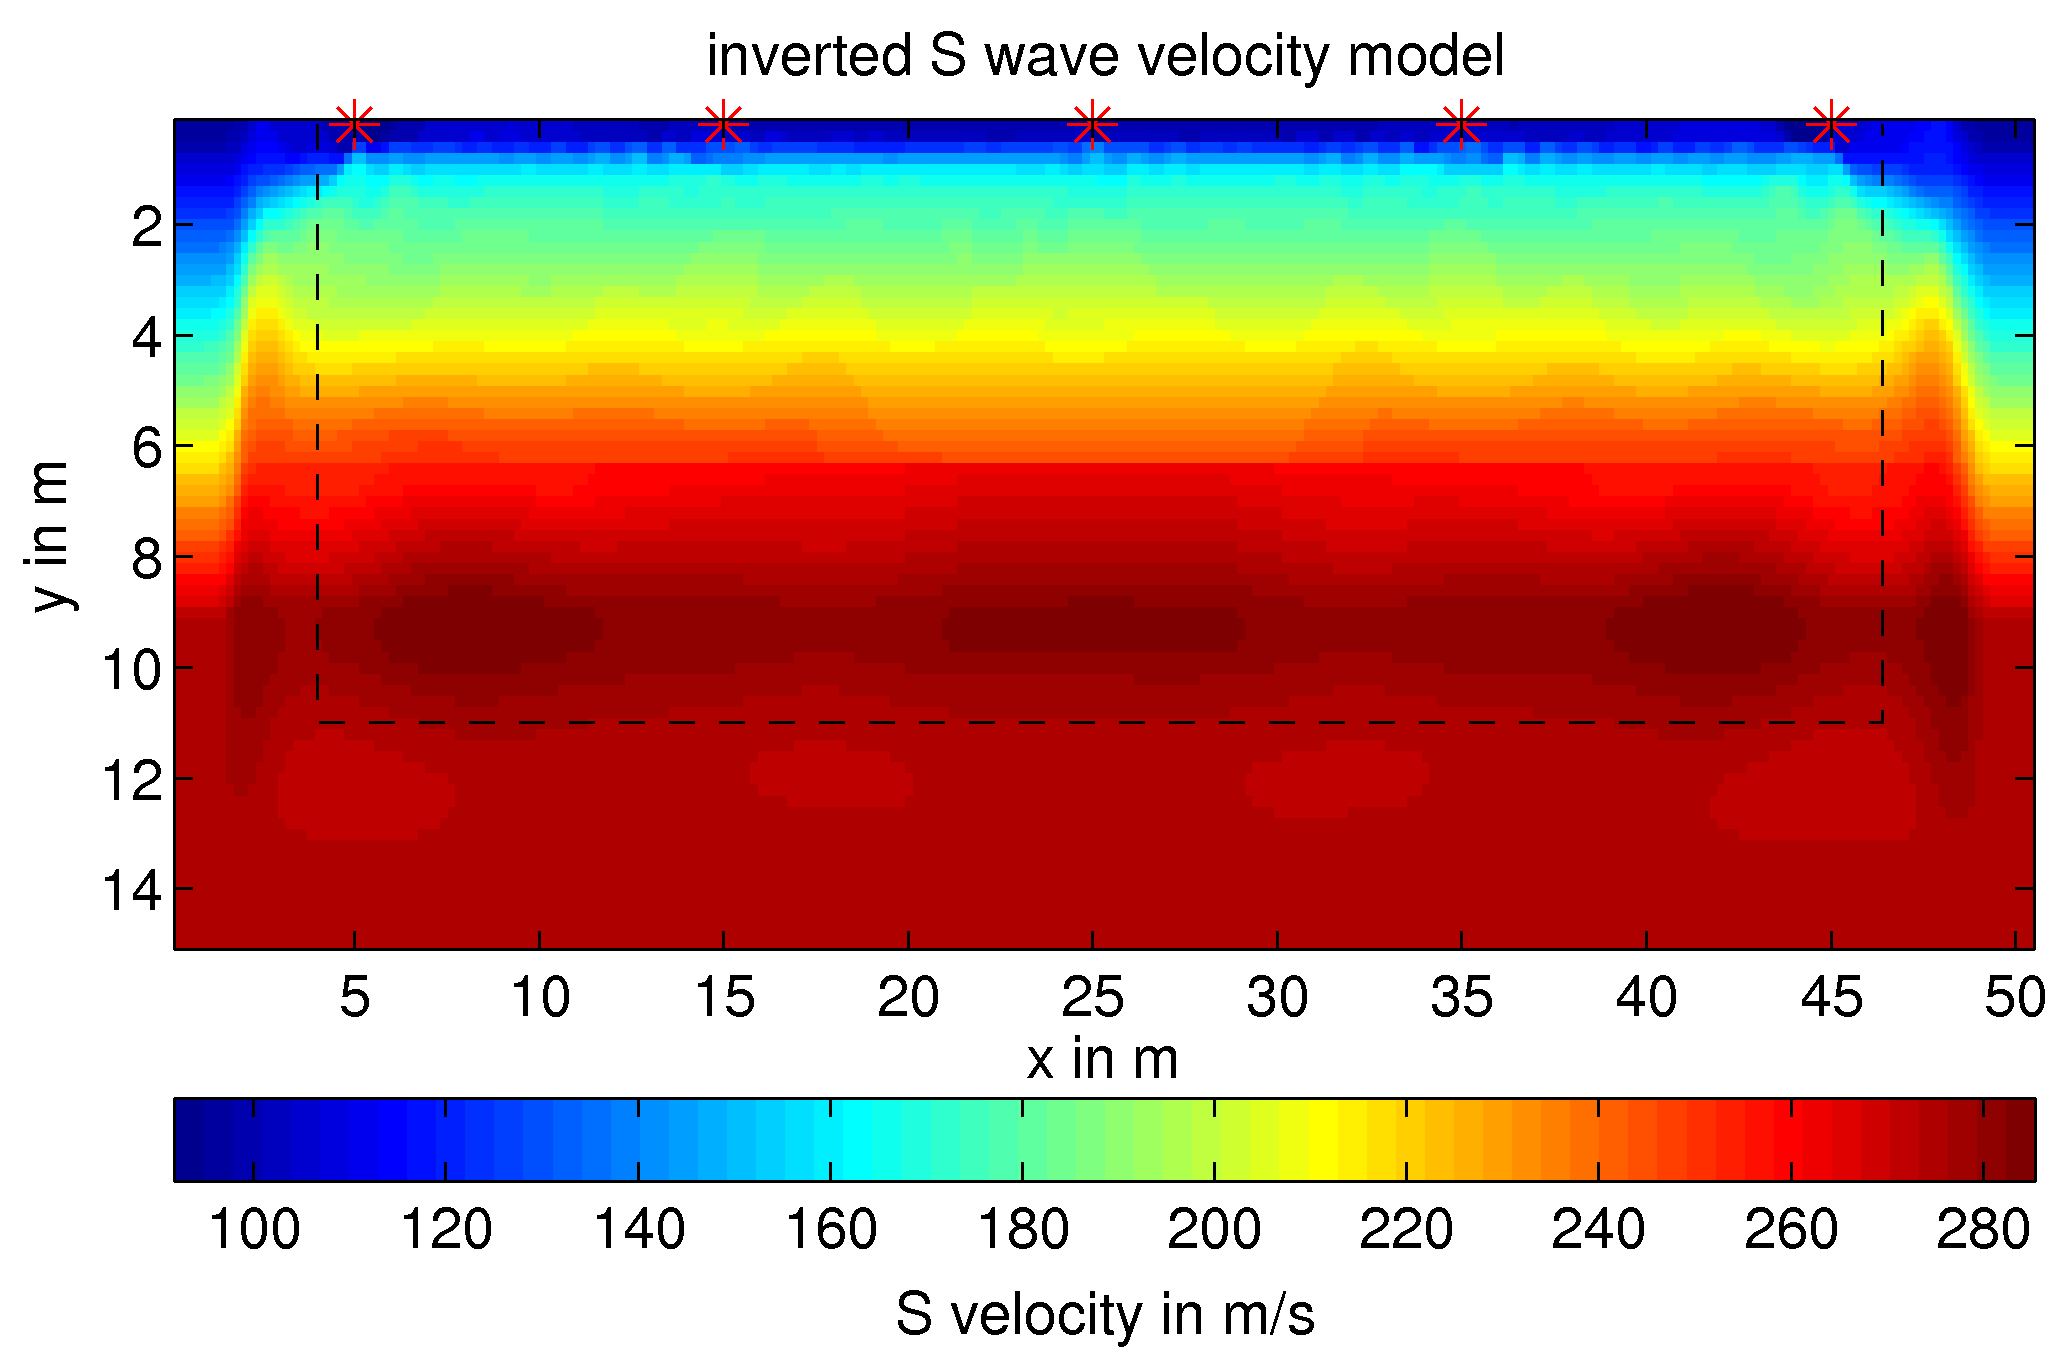
\includegraphics[width=10cm]{figures/Rheinstetten/inv_vs_model}%
\label{inv-vs-model-Rheinstetten}}%
\hspace{0.2 cm}
\subfloat[][]{%
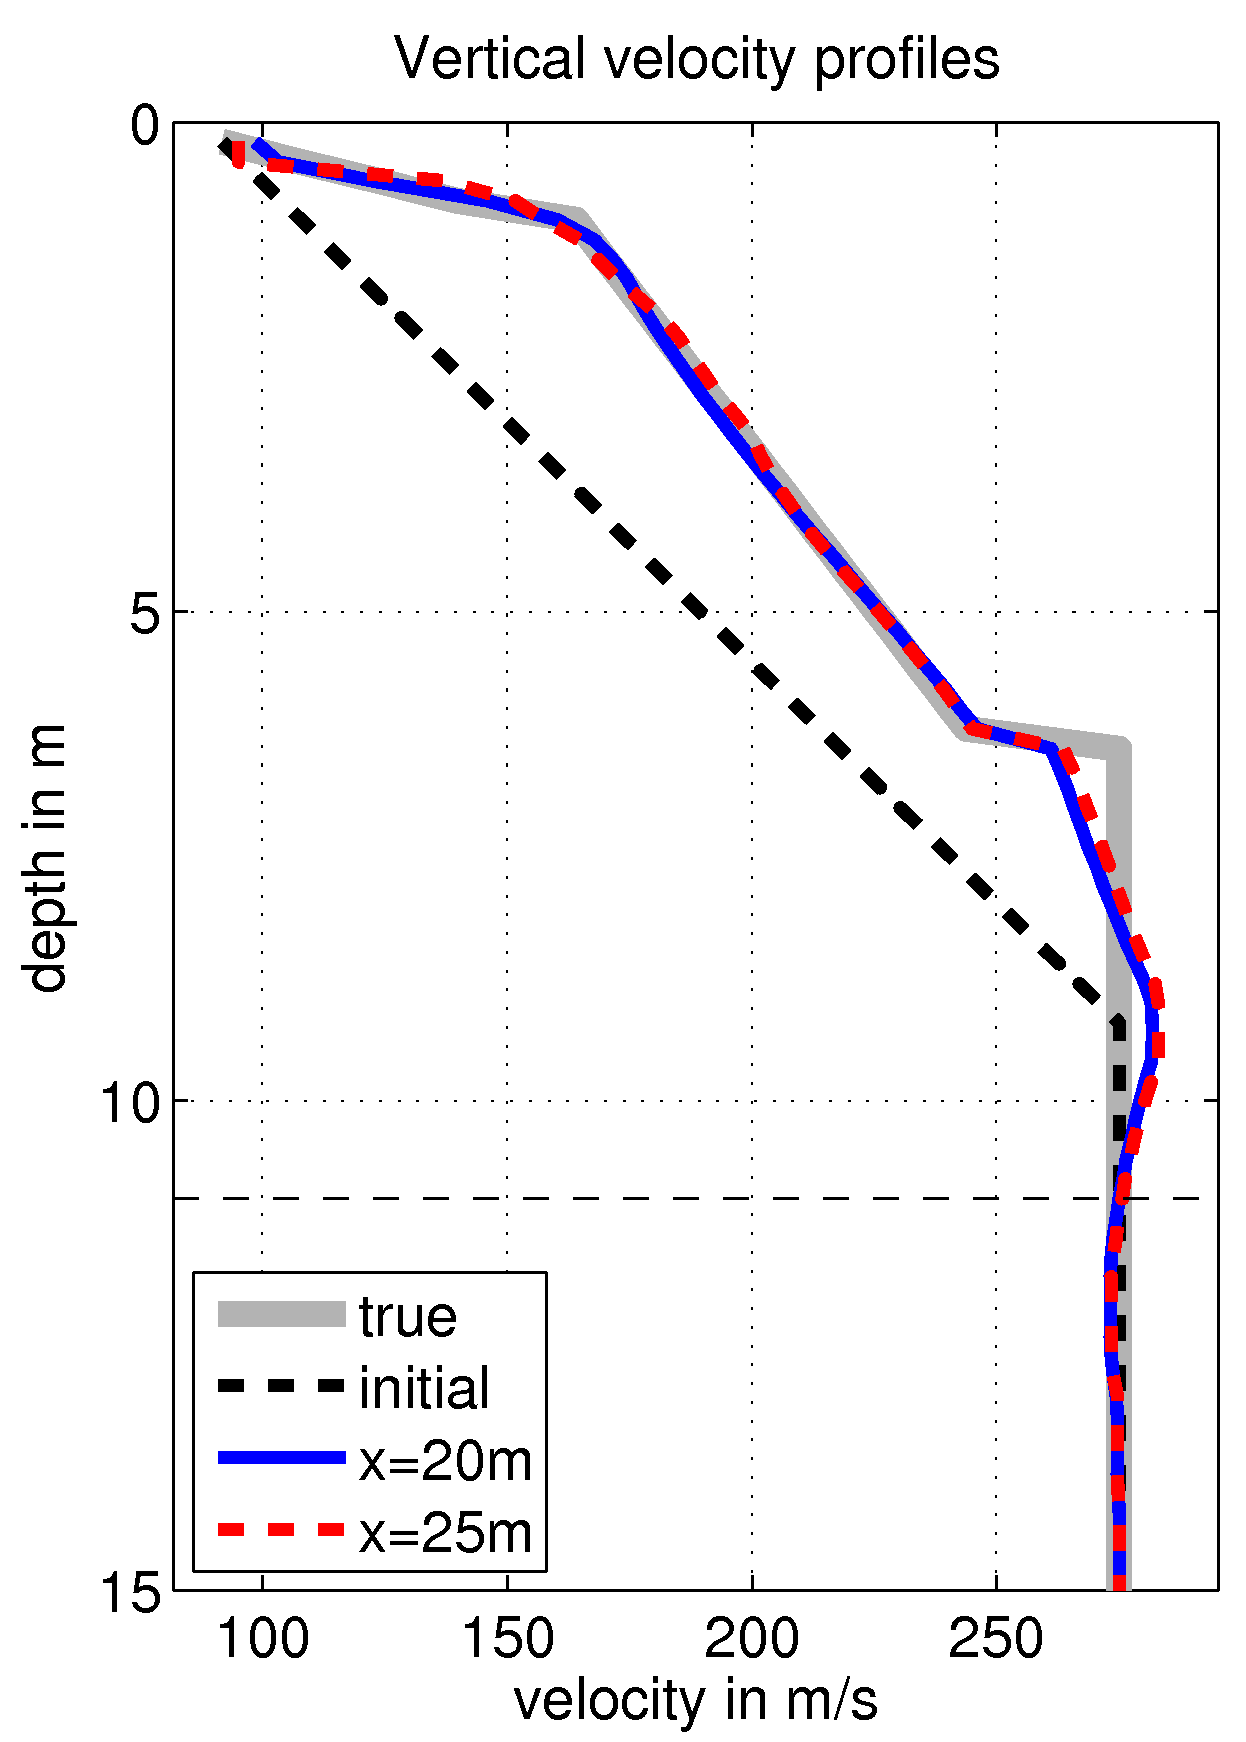
\includegraphics[width=5cm]{figures/Rheinstetten/vertical_vel_profiles}%
\label{vertical-vel-profiles-Rheinstetten}}
\caption{Inverted shear wave velocity model. \protect\subref{inv-vs-model-Rheinstetten} shows an imageplot of the inversion result. The red stars mark the source positions and the black dashed line marks the CPML frame. \protect\subref{vertical-vel-profiles-Rheinstetten} shows vertical velocity profiles of the shear wave velocity models. The true model is plotted with the thick grey line, the initial velocity model is represented by the dashed black line and two vertical profiles at $x$=20\,m and $x$=25\,m of the inverted model are plotted in red and blue. The CPML frame is again marked by the thin black line at 11\,m depth.}
\label{Rheinstetten_inversion_result}
\end{figure}

\clearpage

\section{The complex Marmousi2 model}
\label{complex Marmousi model}
Developed in the 1990s by the French Petroleum Institute (IFP) (\cite{versteeg:94}) the Marmousi model is a widely used test problem for seismic imaging techniques. Beside the original acoustic version of the model an elastic version was developed by \cite{martin:06}. This model consists of parts with simple (approximately 1D) and complex geological situations. In the following two sections the performance of the FWT code will be tested for the complex and the simple part of the Marmousi2 model, respectively.

The Marmousi2 model (Fig. \ref{marmousi_geology}) consists of a 500 m thick water layer above an elastic subseafloor model. The sediment model is very simple near the left and right boundaries but rather complex in the centre. At both sides, the subseafloor is approximately horizontally layered, while steep thrust faults are disturbing the layers in the centre of the model. Embedded in the thrust fault system and layers are small hydrocarbon reservoirs (\FIG{marmousi_geology}, \cite{martin:06}). 
\begin{itemize}
\item One shallow gas sand in a simple structural area (A).
\item One relatively shallow oil sand in a structural simple area (B).
\item Four faulted trap gas sands at varying depths (C1,C2,C3,C4).
\item Two faulted trap oil sands at medium to deep depths (D1,D2).
\item One deep oil and gas sand anticlinal trap (E1,E2).
\item Water wet sand.
\end{itemize}
The deeper parts of the model consist of salt and reef structures. The thrust fault system and the reef structures are not easy to resolve by conventional first arrival tomography, so it is an ideal test model for the FWT. Due to computational restrictions the original Marmousi-II model could not be used, because the very low S-wave velocities in the sediments would require a too small spatial sampling of the model. Therefore new S-wave velocities are calculated using the empirical scaling relation for hard rocks. Additionally the size of the Marmousi2 model is reduced from $\rm{17 \times 3.5\;km}$  to $\rm{10 \times 3.48\; km}$ (\FIG{marmousi_II_true_model}). 
\begin{figure}[!bh]
\centering
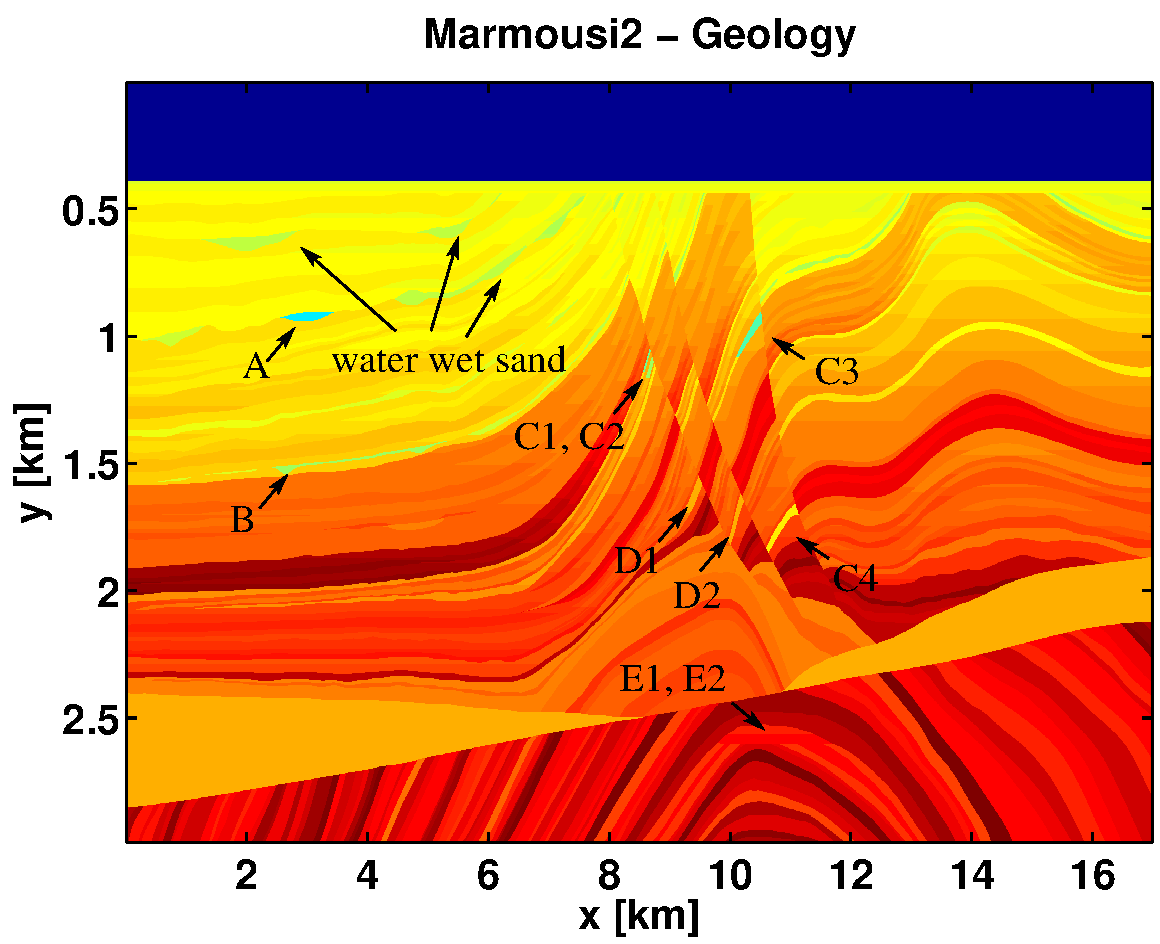
\includegraphics[width=14cm]{figures/marmousi/marmousi_geology.pdf}
\caption{Marmousi2 model - geology.}
\label{marmousi_geology}
\end{figure}
\begin{figure}[!ht]
\centering
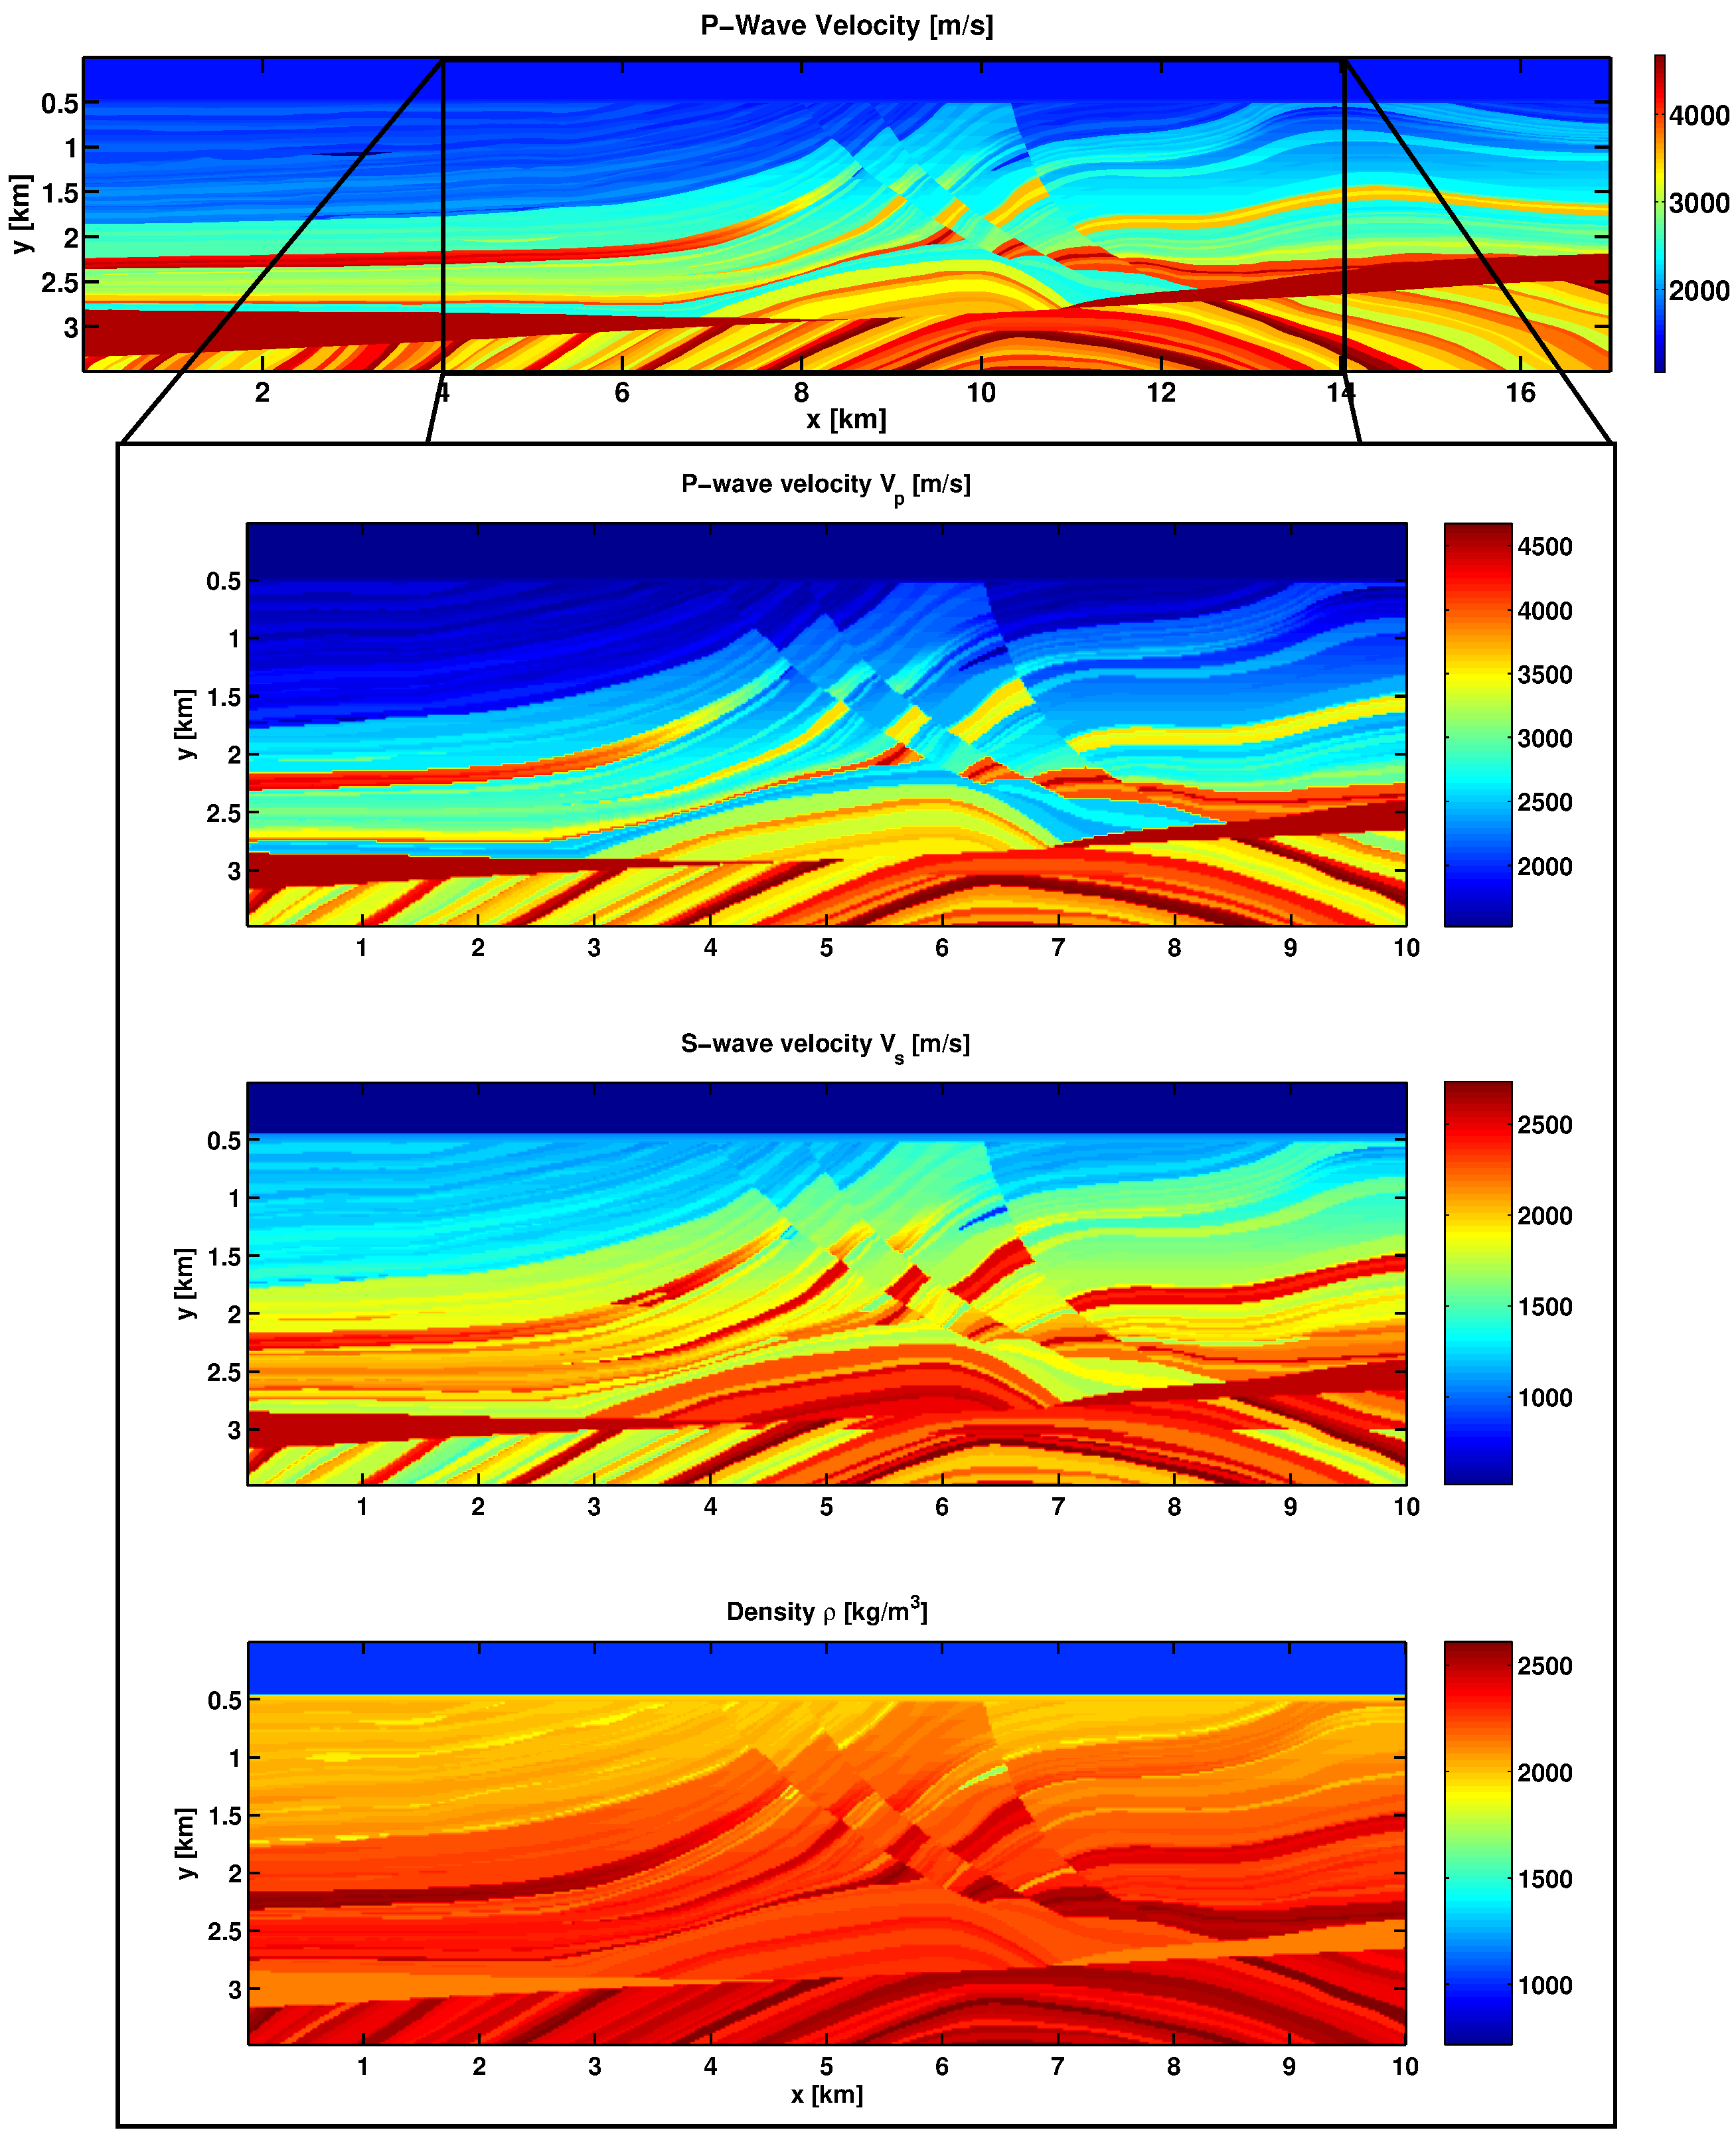
\includegraphics[width=14cm]{figures/marmousi/marmousi_complete_caption.pdf}
\caption{The reduced complex Marmousi2 model used for the elastic FWT.}
\label{marmousi_II_true_model}
\end{figure}
\clearpage\subsection{Acquisition geometry and FD model}
\label{marmousi_acq}
The acquisition geometry consists of a fixed streamer located 40 m below the free surface in the water layer. The streamer contains 400 two component geophones recording the displacements $\rm{u_i}$. For the synthetic dataset 100 airgun shots are recorded. The sources are located at the same depth as the receivers. The source signature is a 10 Hz Ricker wavelet. The model has the dimensions $\rm{10 \times 3.48\; km}$. Using an 8th order spatial FD operator the model can be discretized with $\rm{500 \times 174}$ gridpoints in x- and y-direction with a spatial gridpoint distance of 20.0 m. The time is discretized using DT = 2.7 ms, thus for a recording time of T = 6.0 s 2222 time steps are needed.
\subsection{Elastic wave propagation in the complex Marmousi model}
\label{marmousi_complex}
Fig. \ref{wavefield_marmousi_true} shows the development of the pressure wavefield excited by shot 50 for the central part of the complex elastic Marmousi2 model at 6 different time steps. The P wave is traveling from the source through the water column (T=100.0 ms) and is reflected at the seafloor (T=400.0 ms). In the elastic subseafloor medium the wavefield becomes very complex. The layers in the steep thrust fault system produce numerous reflections and internal multiples (T=600.0 ms). Additionally strong diffracted waves are generated at the sharp corners of the thrust faults between the disturbed high velocity sediment blocks within the thrust faults and the surrounding low velocity sediments. At the free surface strong multiple reflections occur (T=800.0 ms). The wavefront of the direct wave is quite deformed due to strong velocity contrasts within the thrust fault system. After 1500 ms nearly all kinds of waves which can be found in the literature are present: Reflections, refractions, diffractions, (internal) multiples or interface waves. The trapped gas sand reservoirs C1, C2 and C3 produce strong reflections and mode conversions. This complexity is also visible in the seismic section, recorded by the streamer in the water column. As an example Fig. \ref{marmousi_seis}, (f) shows the seismic section of the y-component for shot 50. Beside the direct wave and a strong reflection from the seafloor numerous small reflection events from the thrust fault system are dominating the seismic section.  
\begin{figure}
\begin{center}
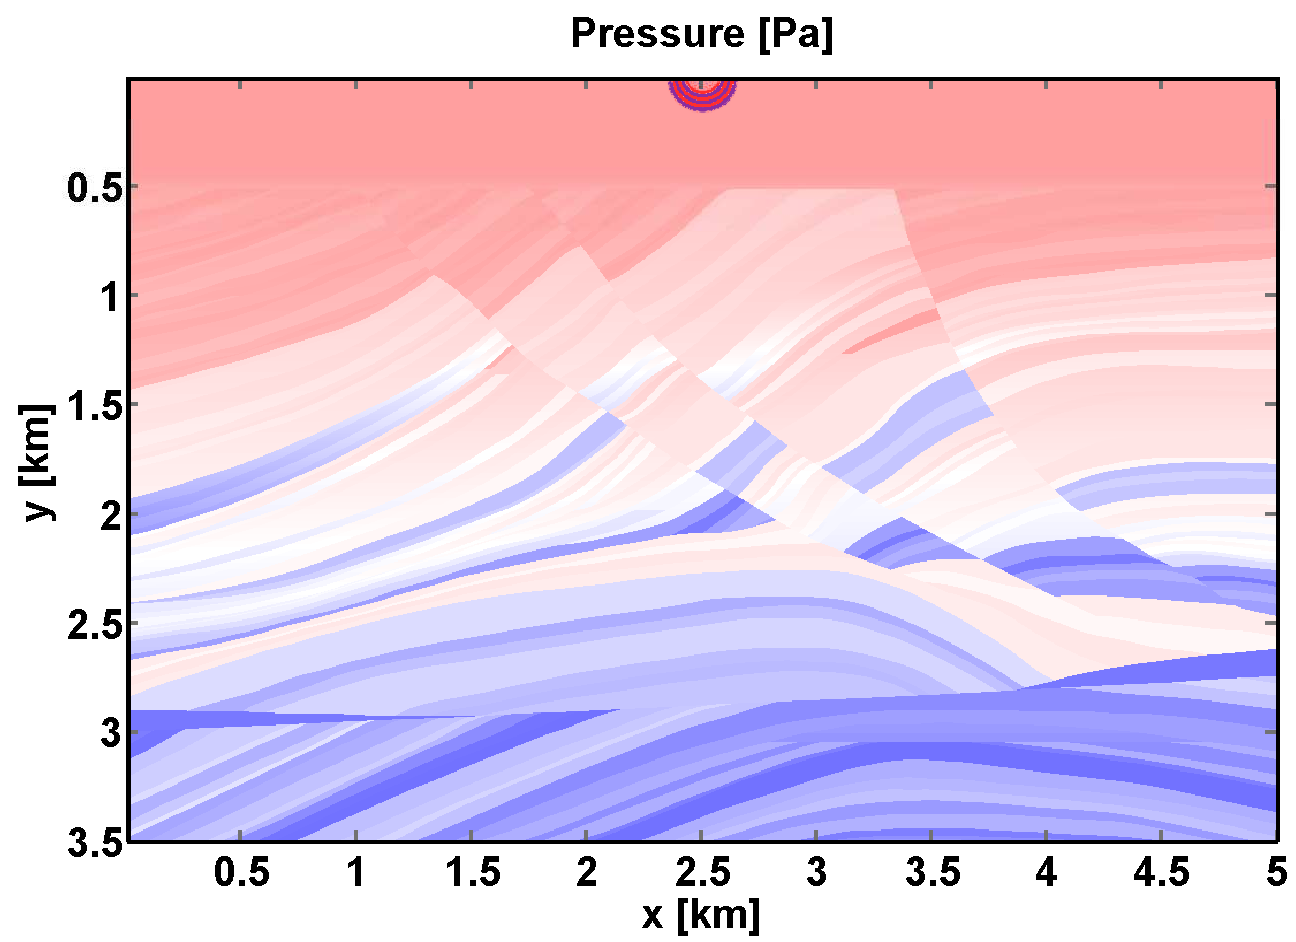
\includegraphics[width=7.5cm]{figures/marmousi/shot93_snap_2.pdf}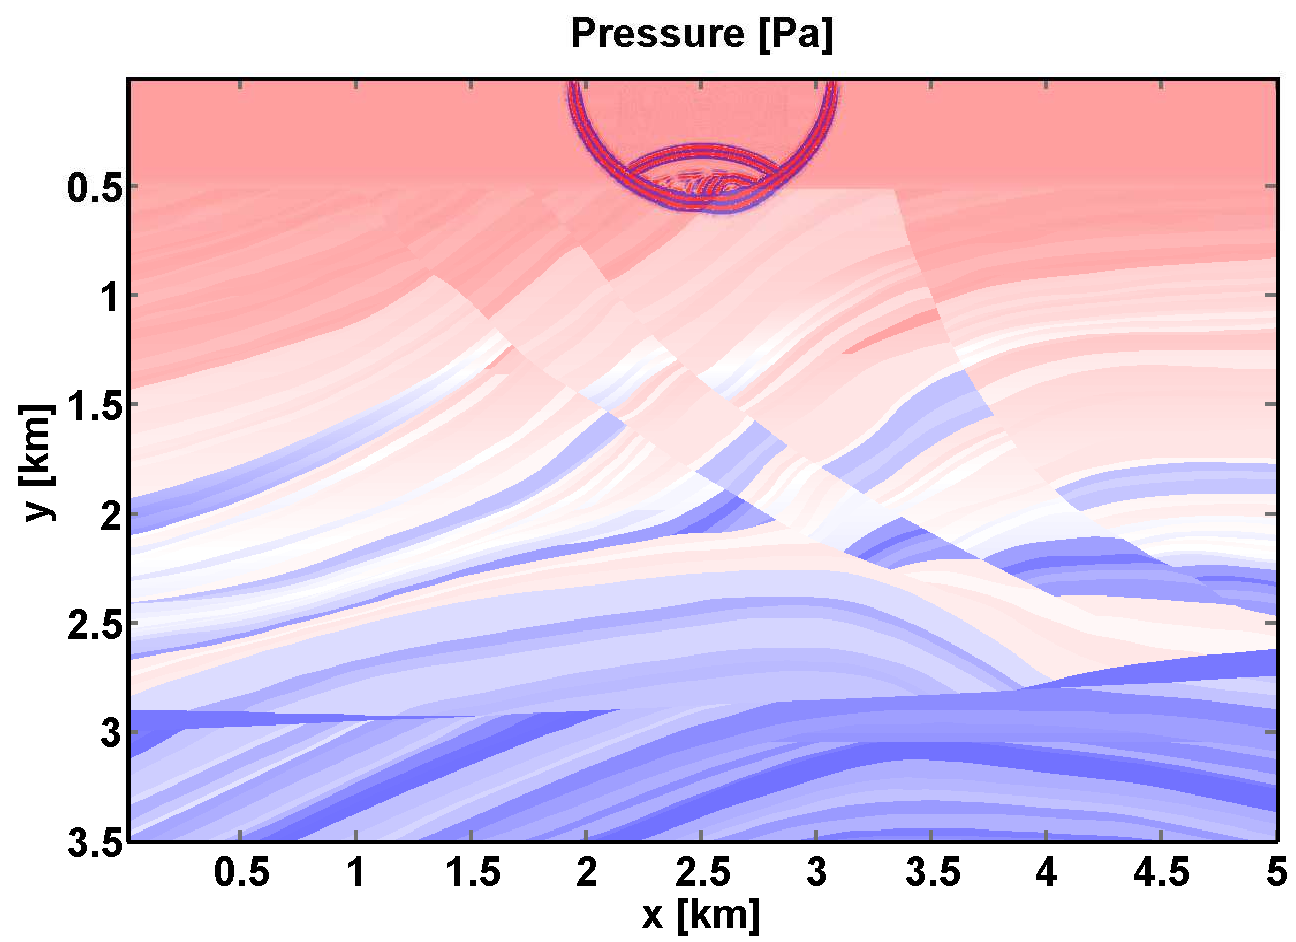
\includegraphics[width=7.5cm]{figures/marmousi/shot93_snap_5.pdf}\\ 
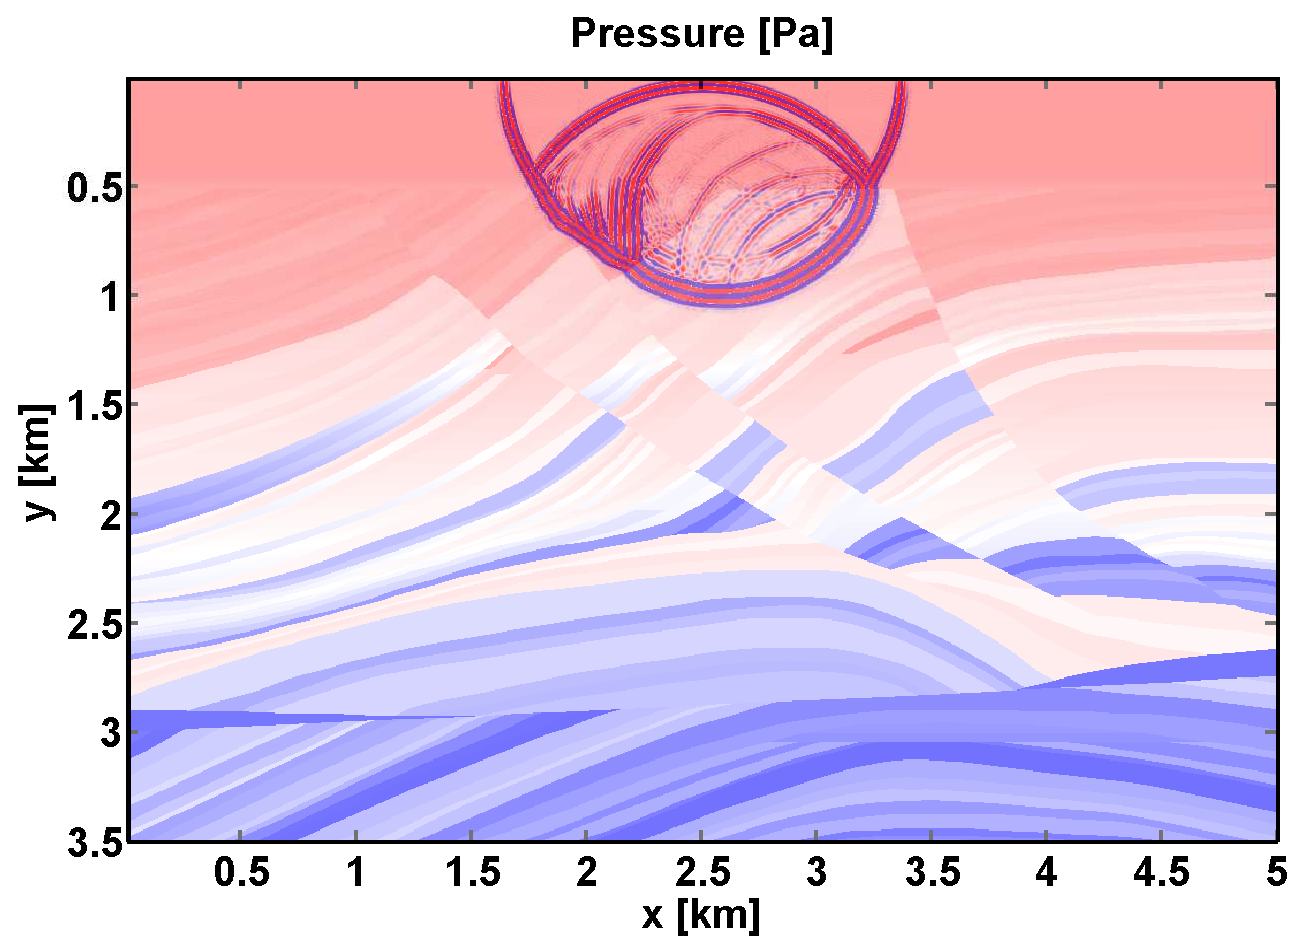
\includegraphics[width=7.5cm]{figures/marmousi/shot93_snap_7.pdf}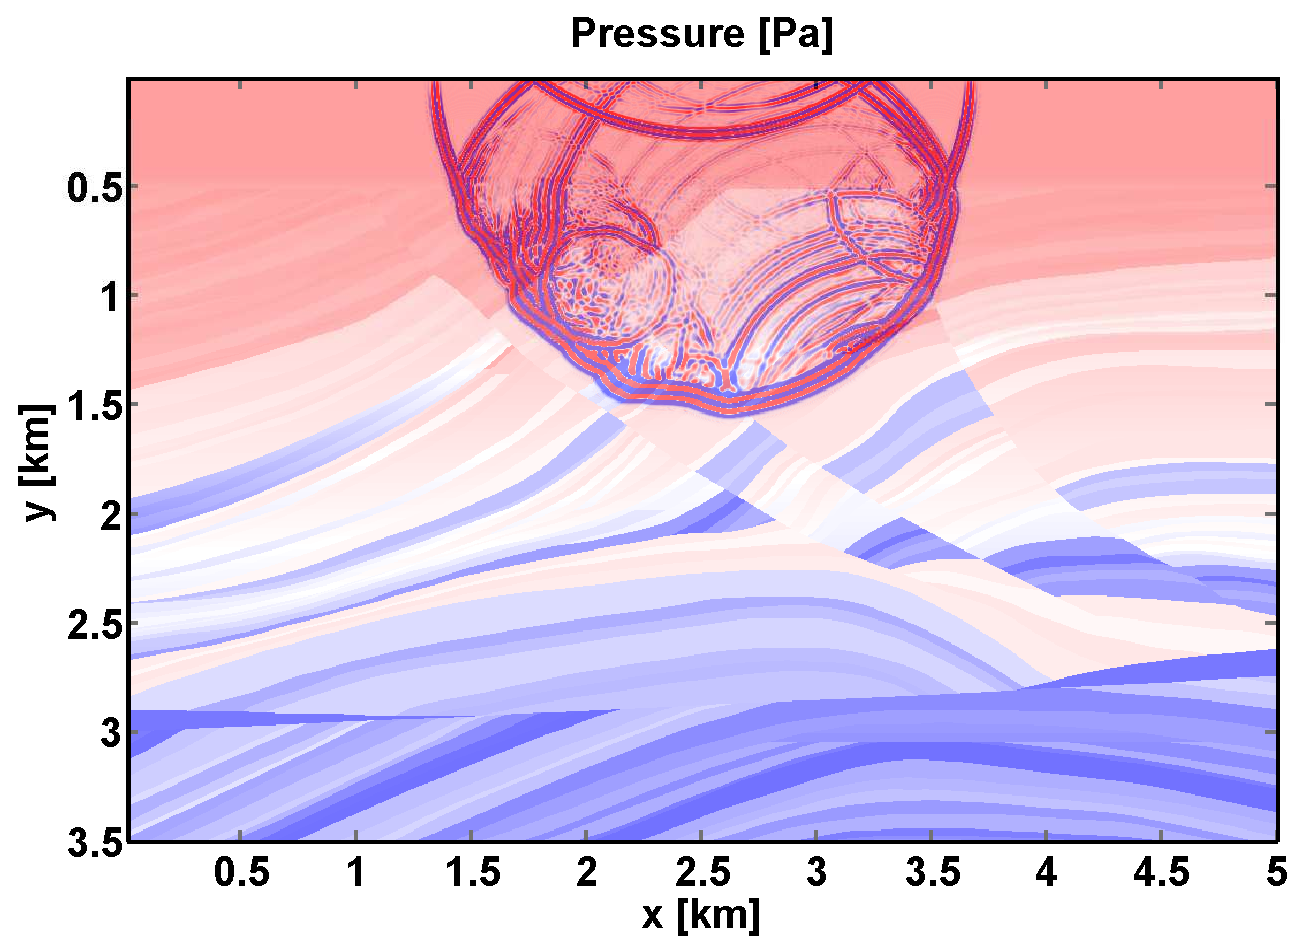
\includegraphics[width=7.5cm]{figures/marmousi/shot93_snap_9.pdf}\\ 
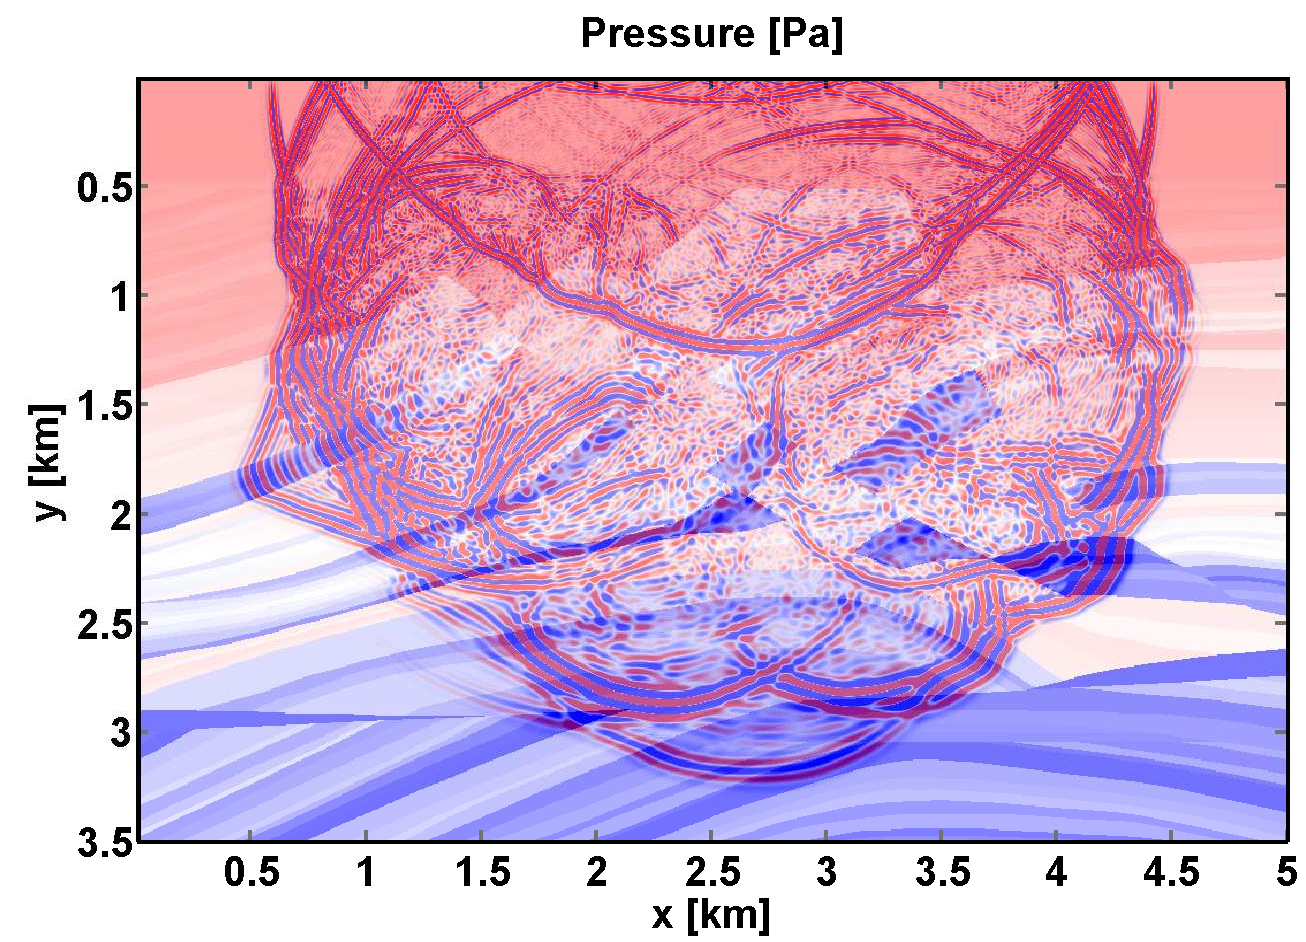
\includegraphics[width=7.5cm]{figures/marmousi/shot93_snap_14.pdf}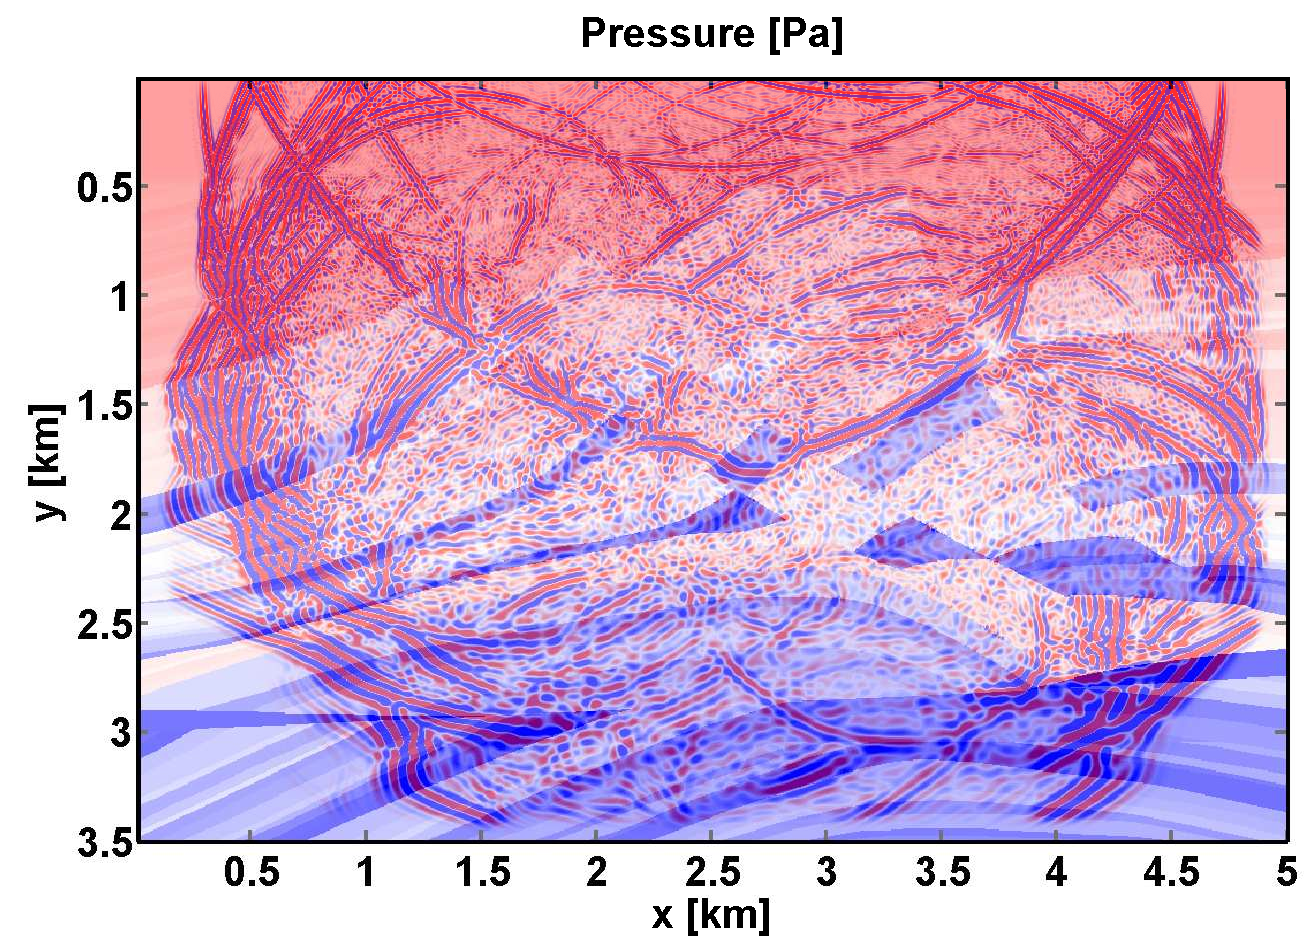
\includegraphics[width=7.5cm]{figures/marmousi/shot93_snap_16.pdf}\\ 
\caption{Pressure wavefield excited by shot 50 for the elastic Marmousi2 model at 6 different time steps .}
\label{wavefield_marmousi_true}
\end{center}
\end{figure}
\clearpage
\subsection{FWT of the complex Marmousi model}
\label{marmousi_complex_FWT}   
Due to the results of the last section, I choose the seismic velocities as model parameters for the inversion. To generate a starting model which describes the long wavelength part of the material parameters correctly the true model $\rm{\mathbf{m}=[V_p,\;V_s,\;\rho]}$ was filtered using a spatial 2D-Gaussian filter 
\begin{equation}
\rm{\mathbf{m}_{smooth}(x,y) = \frac{1}{2 \pi \lambda_c^2} \int_{-\lambda_c}^{\lambda_c} \int_{-\lambda_c}^{\lambda_c} dx' dy' \mathbf{m}(x-x',y-y') exp\biggl(-\frac{(x-x')^2+(y-y')^2)}{2 \lambda_c^2}\biggr)}
\label{gaussian}
\end{equation}
with a correlation length $\rm{\lambda_c = 200.0\;m}$. As a result all the small scale structures vanished and only the large scale structures are present (Fig. \ref{marmousi_II_start}). 
\begin{figure}[!bth]
\begin{center}
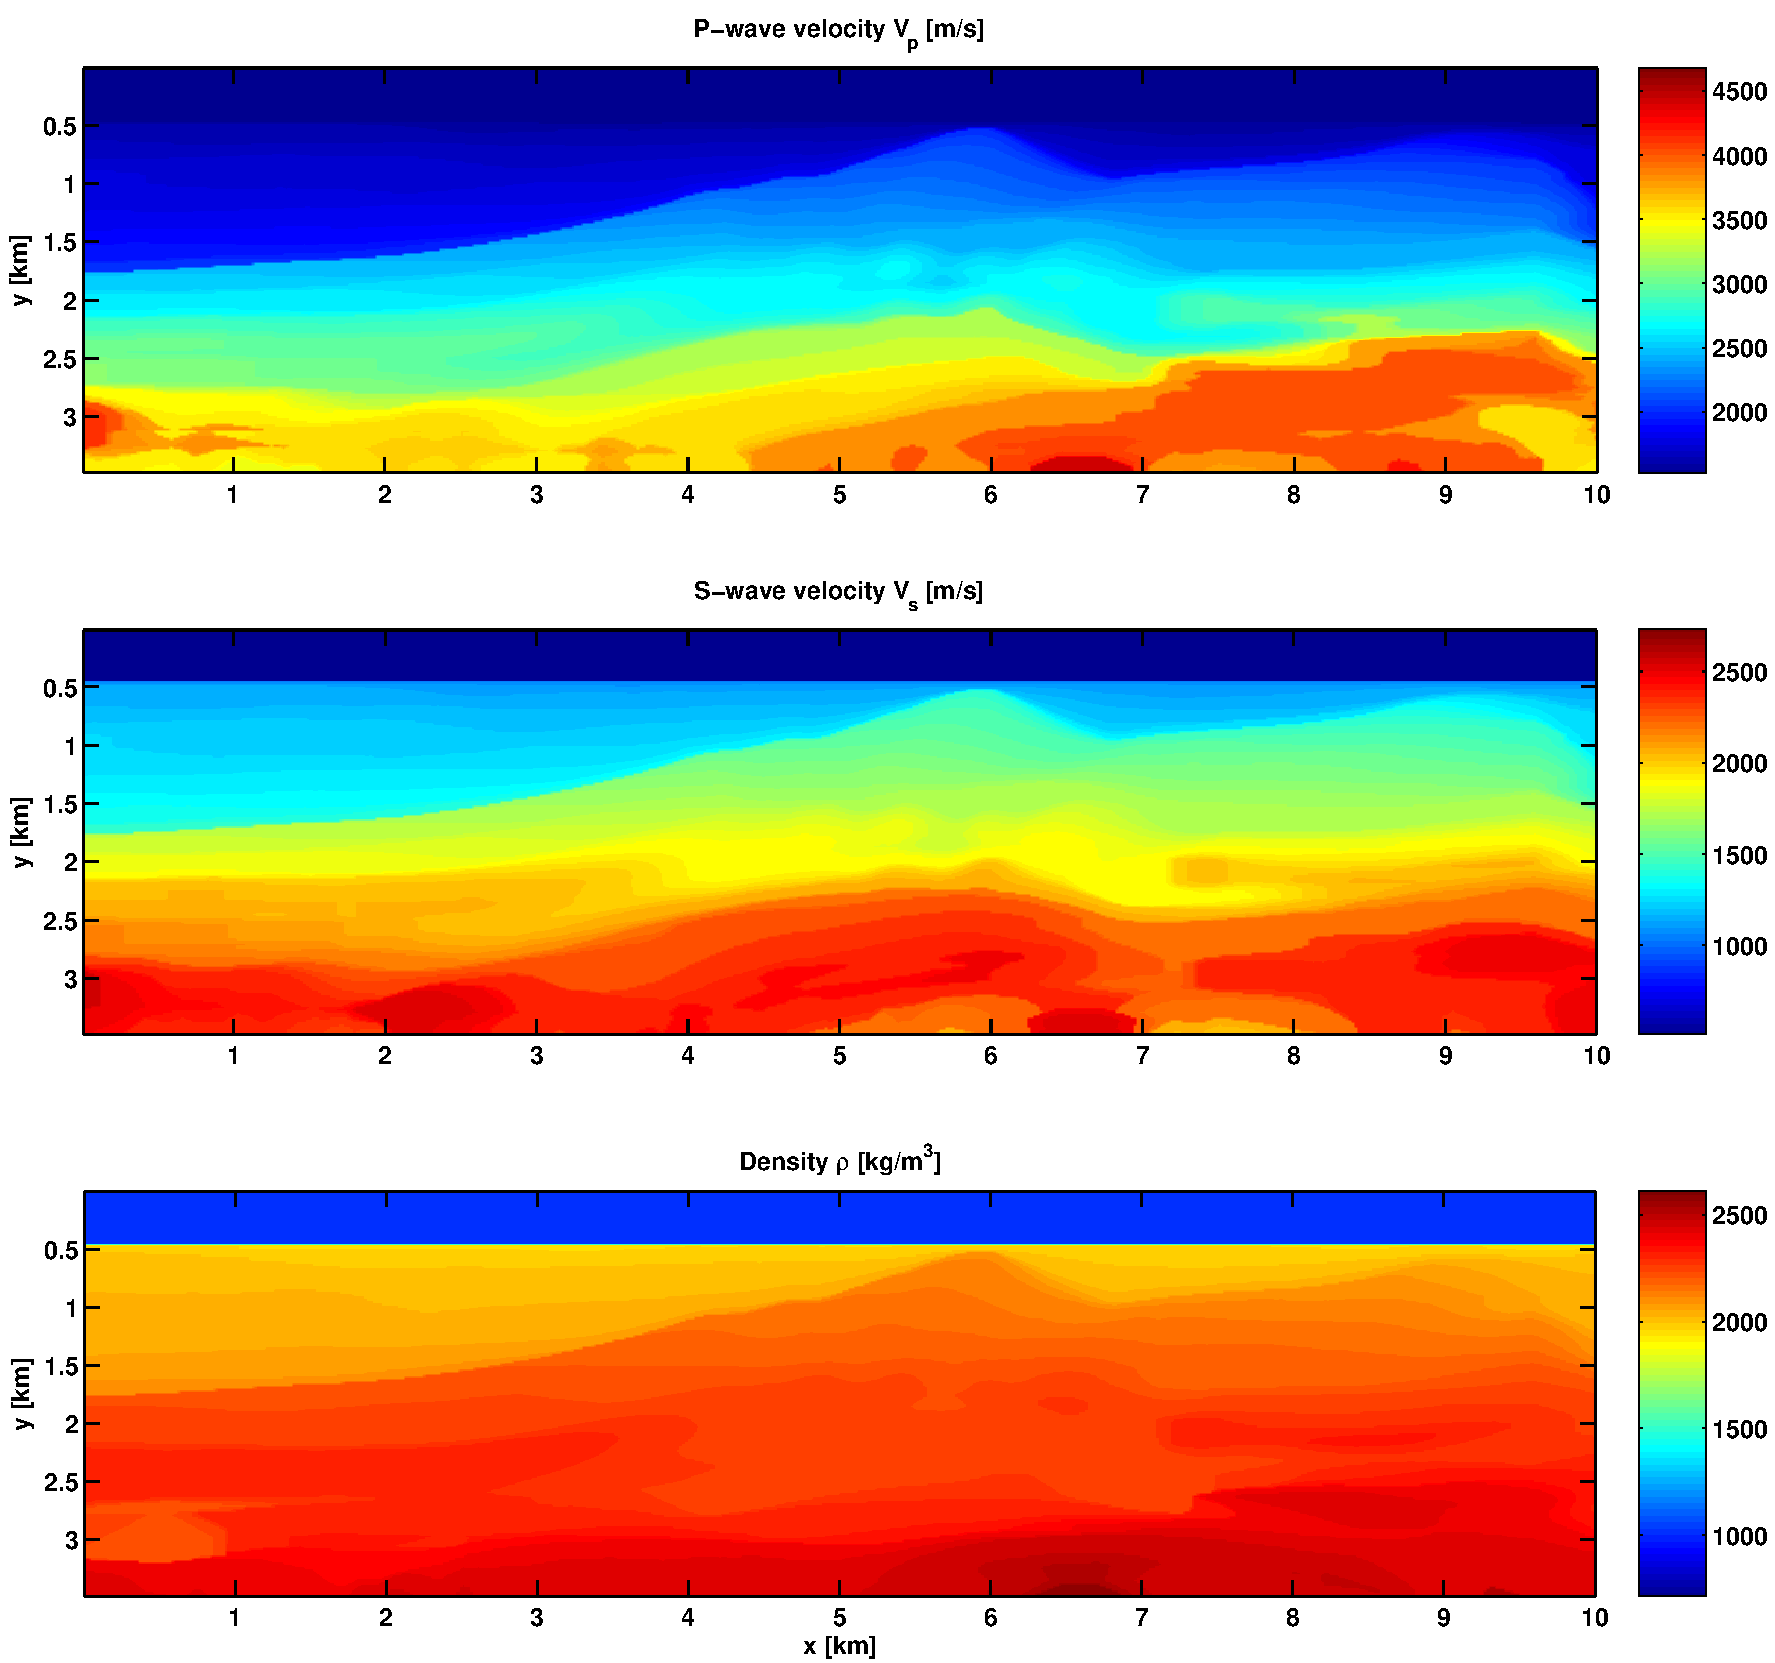
\includegraphics[width=12cm]{figures/marmousi/marmousi_II_start.pdf}
\caption{Starting models for the Marmousi-II model.}
\label{marmousi_II_start}
\end{center}
\end{figure}
\clearpage
As in the case of the spherical low velocity anomaly the application of a preconditioning operator is vital to suppress the large gradient values near the source and receiver positions. Additionally strong artefacts are present near the free surface (\FIG{marmousi_II_precond}, top) which are a few orders of magnitude larger than the gradient of the material parameters. This problem is also known in case of the acoustic inversion problem (\cite{benhadj:2008}).  To suppress these effects a spatial preconditioning operator is applied on the gradient, which is defined as (\FIG{taper_grad_marm})
\EQ{marmousi_prec:1}{\rm{P=}
\begin{cases}
\rm{0} & \text{if } \rm{y_0 = 0.0\; m} \le y \le \rm{y_{gradt1} = 380.0\; m}\\
\rm{exp(-\frac{1}{2}(a\frac{y-y_{gradt1}-\Delta l}{\Delta l/2})^2)} & \text{if } \rm{y_{gradt1} = 380.0\; m} \le y \le \rm{y_{gradt2} = 480.0\; m}\\
\rm{\frac{y}{y_{gradt2}}} & \text{if } \rm{y_{gradt2} = 480.0\; m} < y \\
\end{cases}}
with $\rm{a=3.0}$, $\rm{\Delta l=100.0\;m}$. \\
\begin{figure}[!ht]
\begin{center}
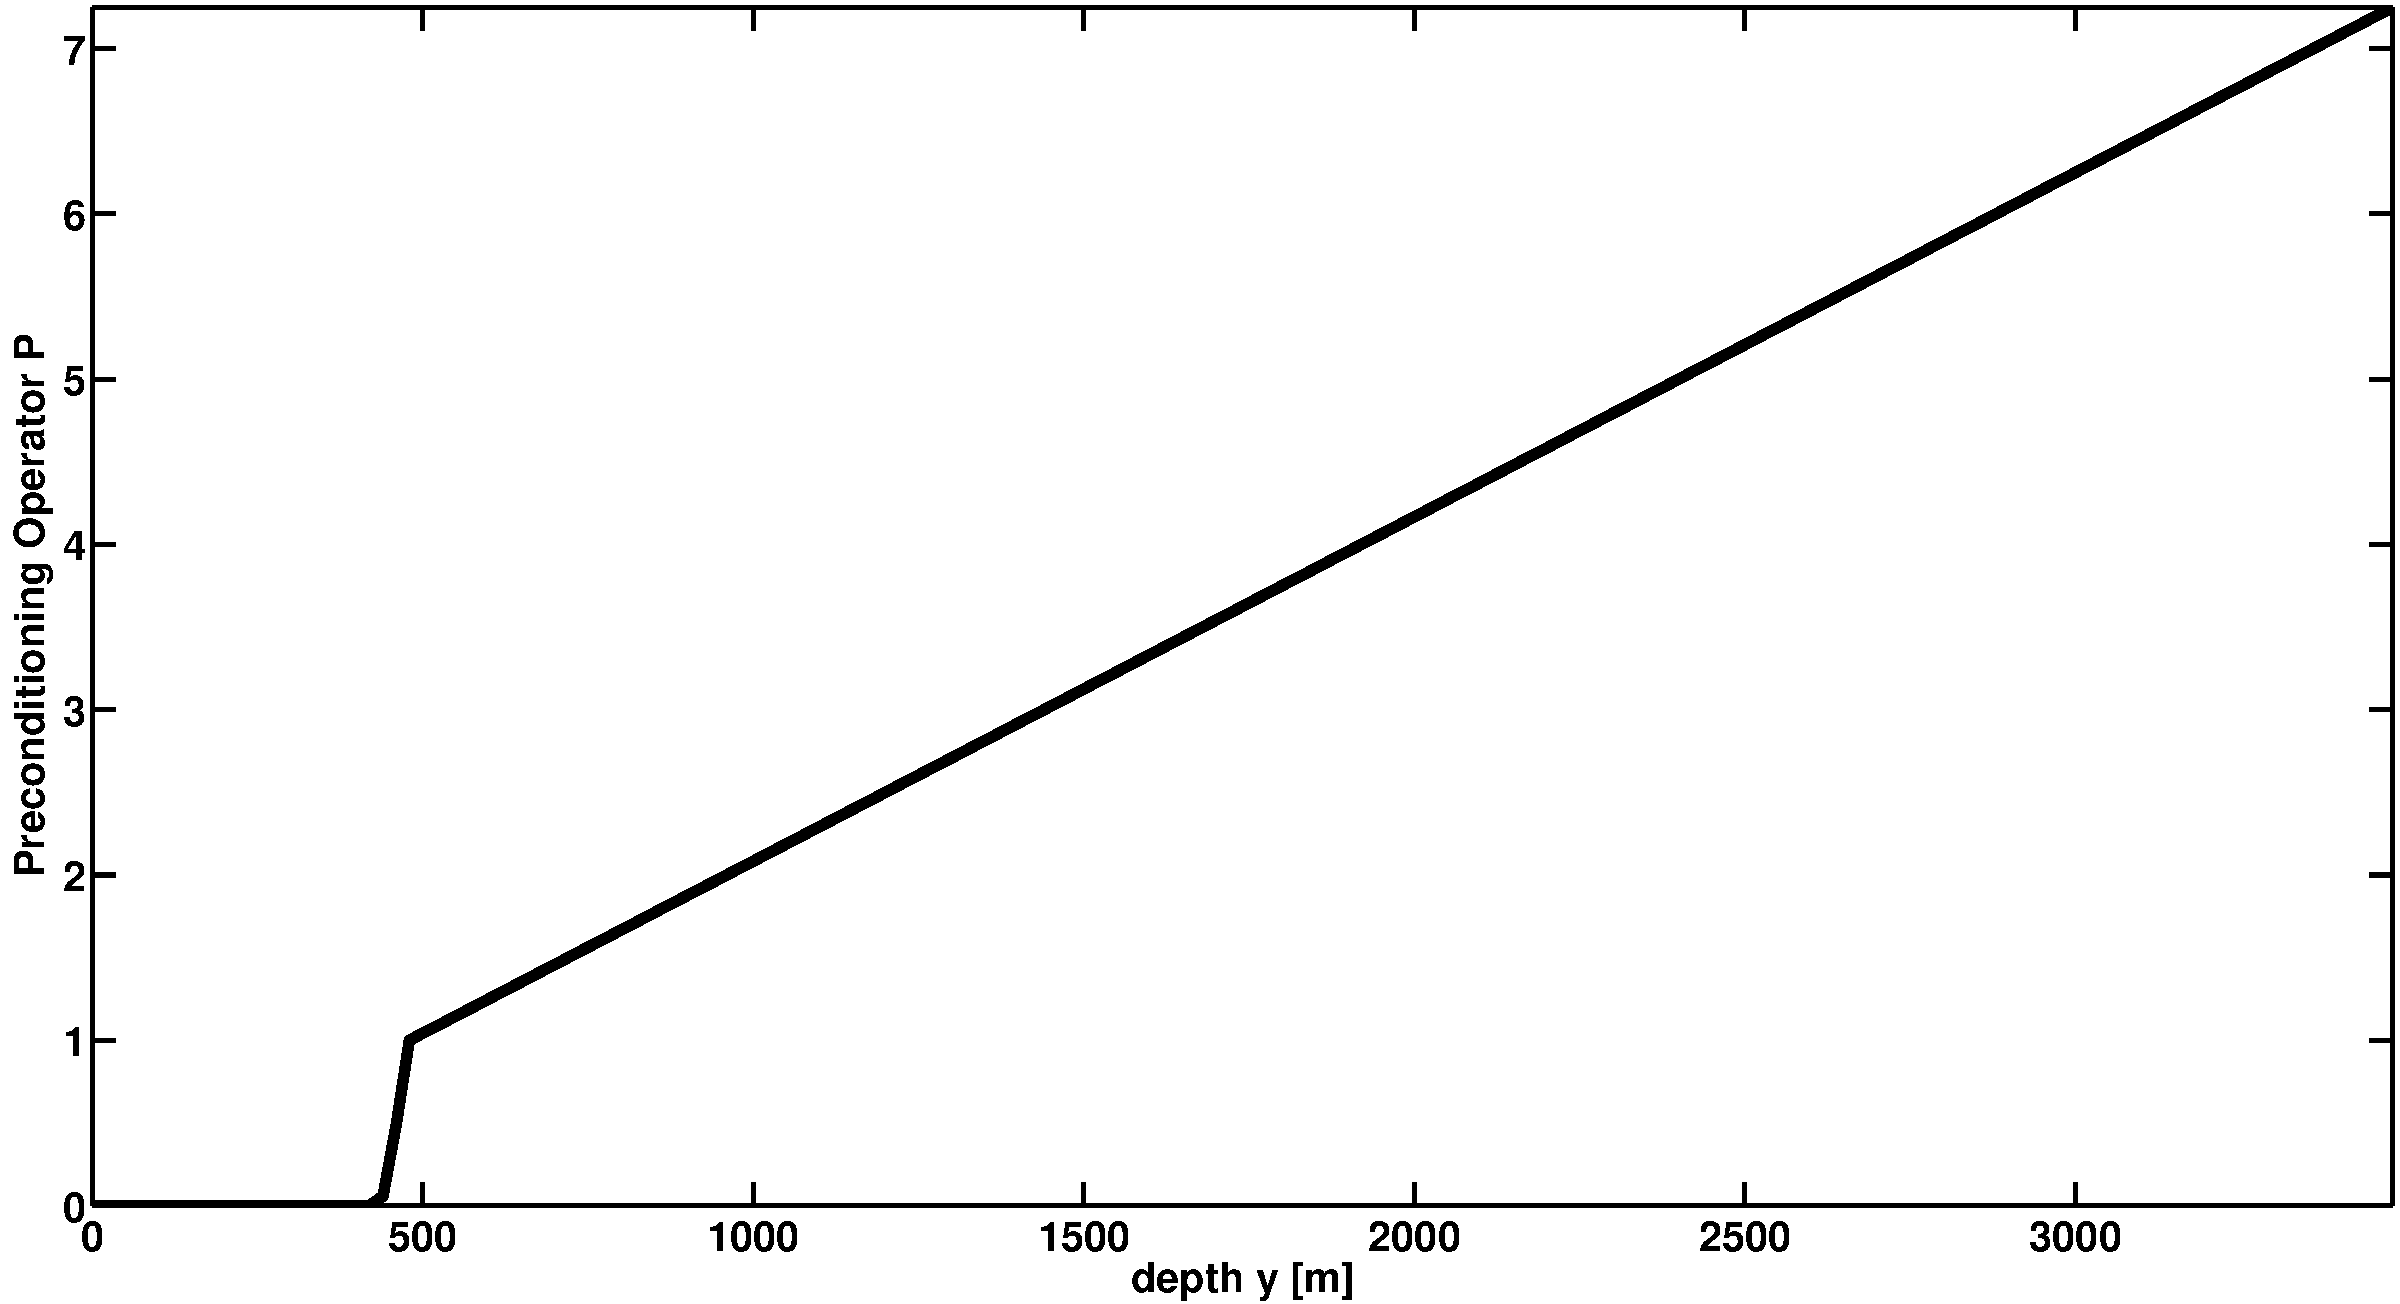
\includegraphics[width=12cm]{figures/marmousi/taper_grad_refl.pdf}
\caption{The preconditioning operator for the reflection geometry.}
\label{taper_grad_marm}
\end{center}
\end{figure}
The preconditioning operator sets the gradient near the free surface and the sources/receivers to zero. In a transition zone between 380.0 m and 480.0 m depth a Gaussian taper is applied. Beyond a depth of 480 m the operator scales the gradient linear with depth. This is a very crude correction for the amplitude loss in larger depths due to geometrical spreading and reflections in the upper parts of the model. Before the application of the preconditioning operator no subsurface structures are visible at all \FIG{marmousi_II_precond} (top), while strong reflectors are visible after its application.
\clearpage      
\begin{figure}[!bth]
\begin{center}
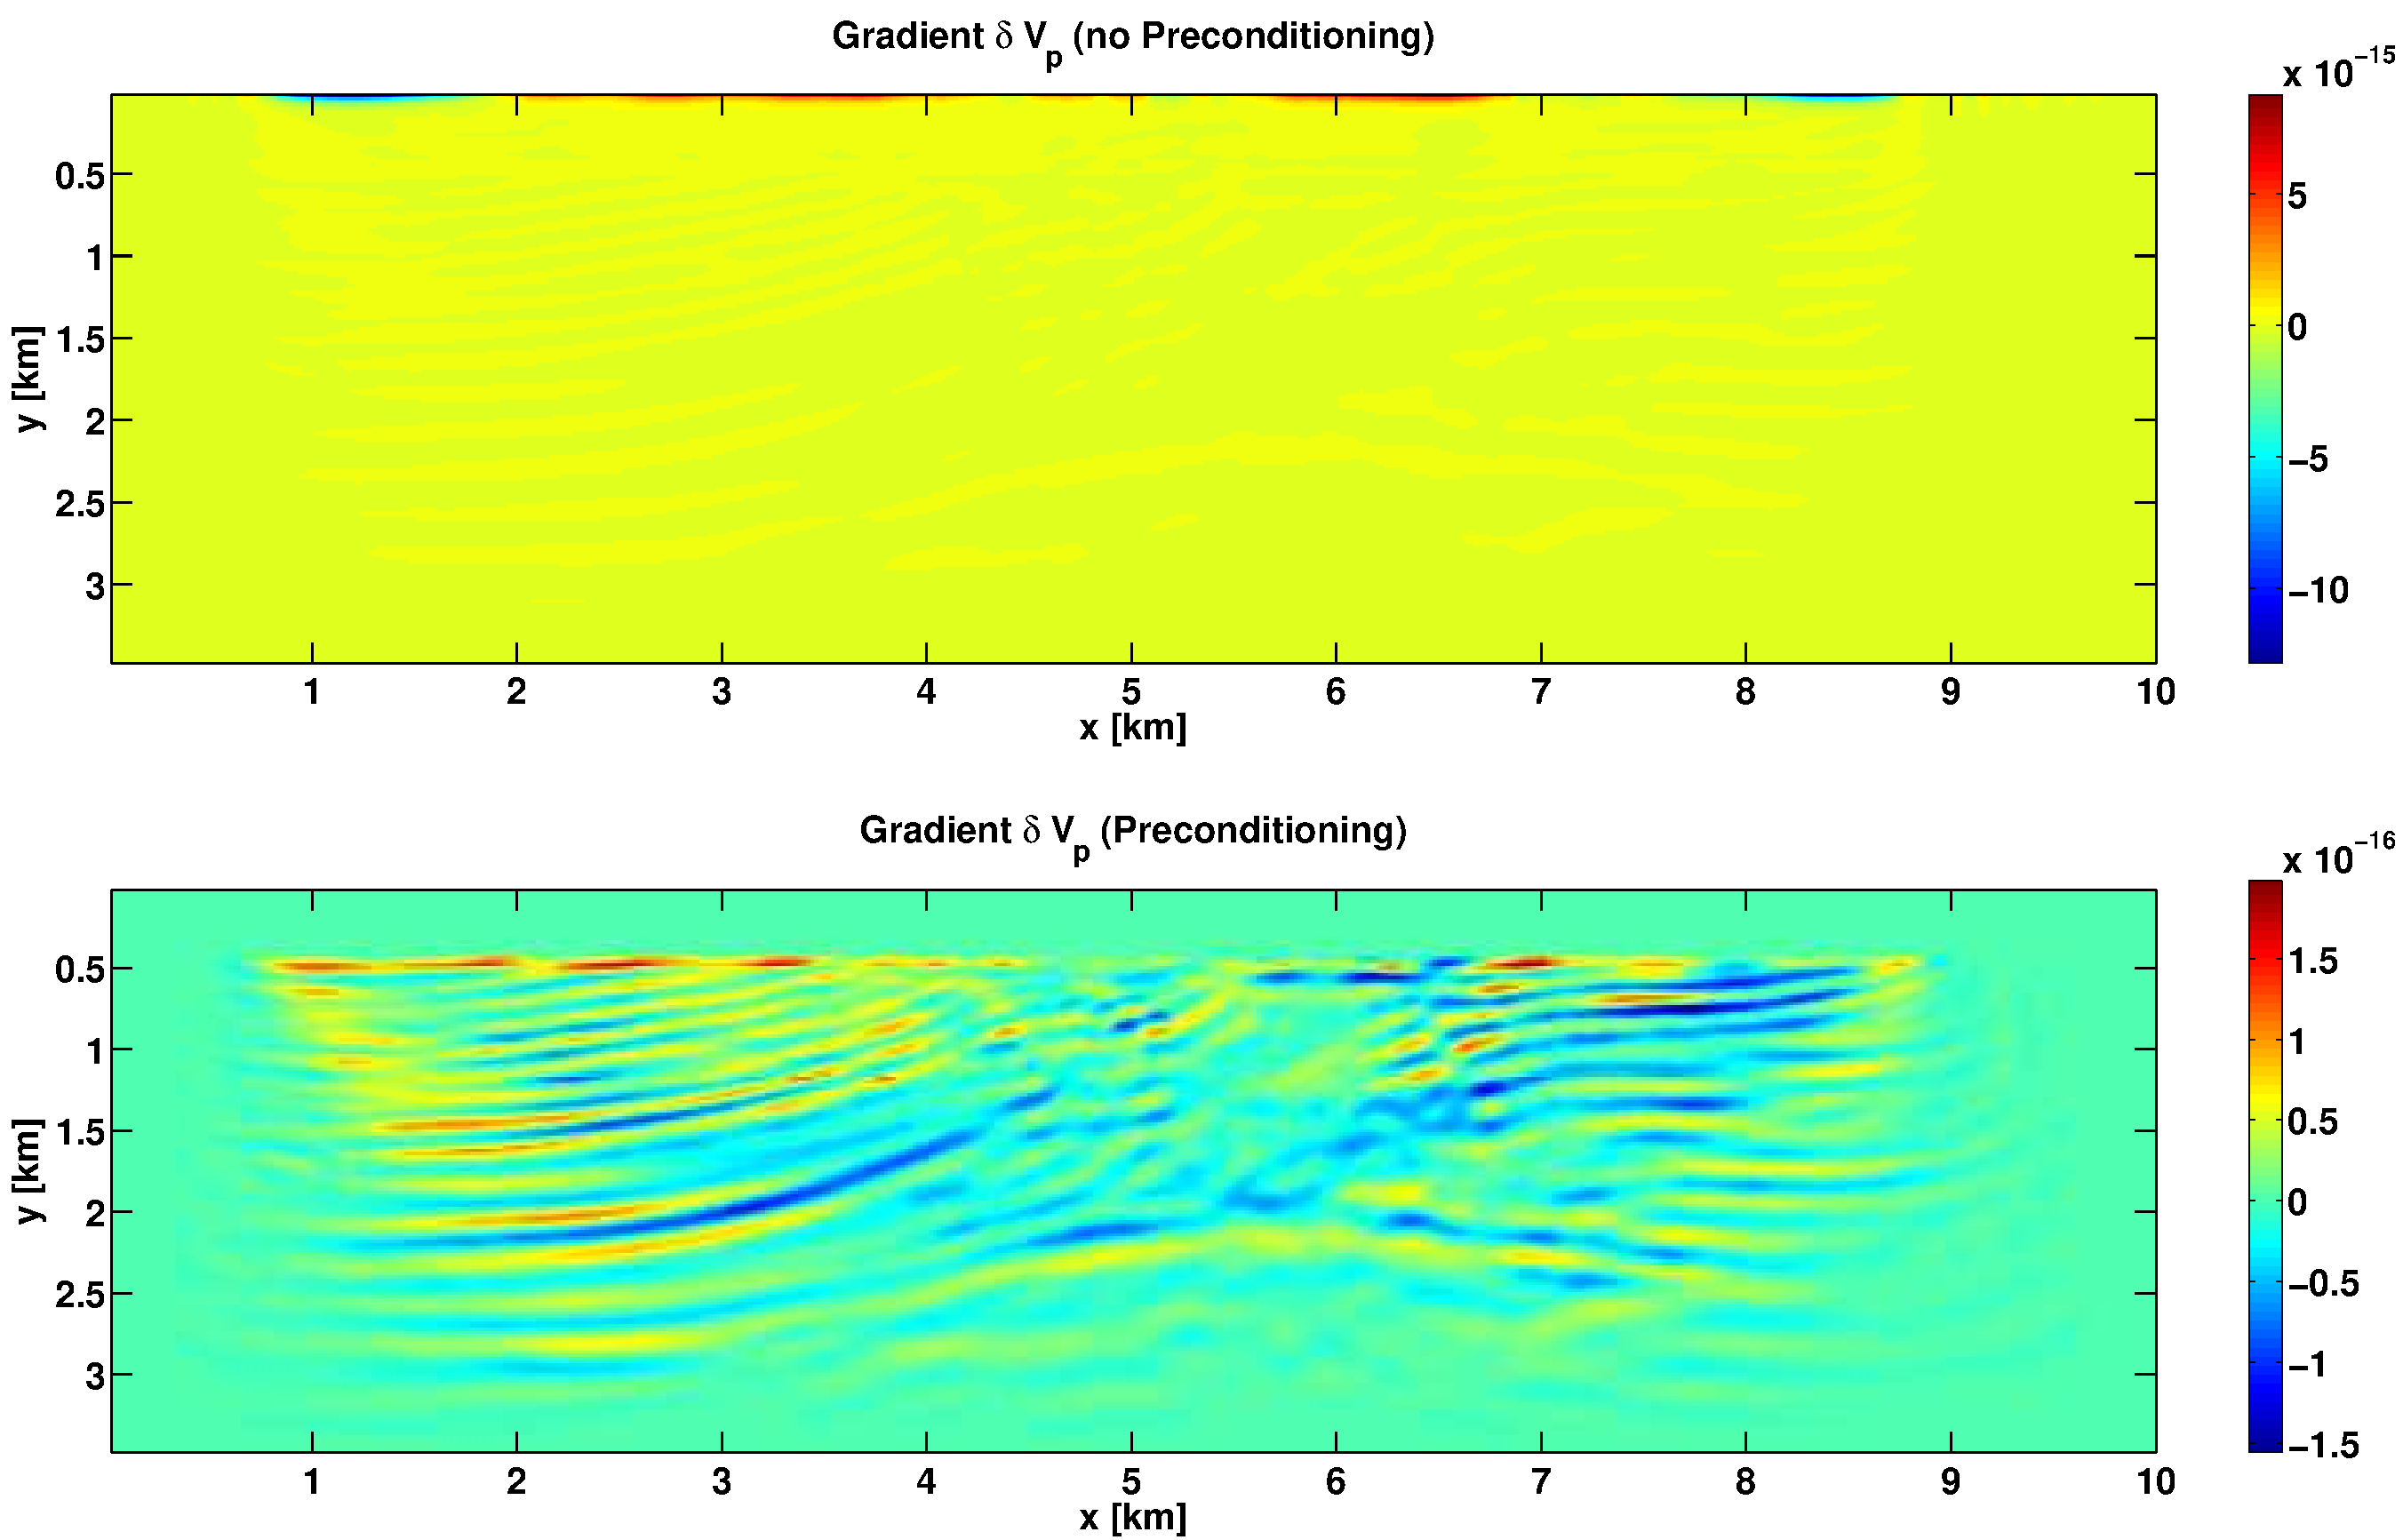
\includegraphics[width=15cm]{figures/marmousi/marmousi_II_precond.pdf} 
\caption{The influence of the preconditioning operator P for the elastic Marmousi2 model. The Gradient $\rm{\delta V_p}$ (iteration no. 1) before (top) and after the application of the preconditioning operator (bottom).}
\label{marmousi_II_precond}
\end{center}
\end{figure}  
To achieve a smooth transition from the long wavelength starting model to the inversion result with short wavelength structures the application of a frequency filter with variable bandwidth on the data residuals $\rm{\delta \mathbf{u}}$ is vital, to avoid the convergence into a local minimum. In this case the inversion is separated in two parts. In part I only frequencies below 10 Hz are inverted, while in part II the full spectral content up to 20 Hz is inverted. The inversion results after 350 iterations are shown in Fig. \ref{marmousi_II_result}. Additionally depth profiles at $\rm{x_{p1}=3.5\;km}$ and $\rm{x_{p2}=6.4\;km}$ of the starting model and inversion result are compared with the true model in Fig. \ref{marmousi_II_result_profile}. The results contain a lot of small details. All fine layers which are completely absent in the starting model could be resolved. The thrust faults and the reef structures in the deeper part of the model are imaged also very well. Despite the deep hydro carbon reservoirs E1 and E2, the oil and gas reservoirs C1, C2, C3, C4, D1 and D2 are all clearly visible.
\begin{figure}
\centering
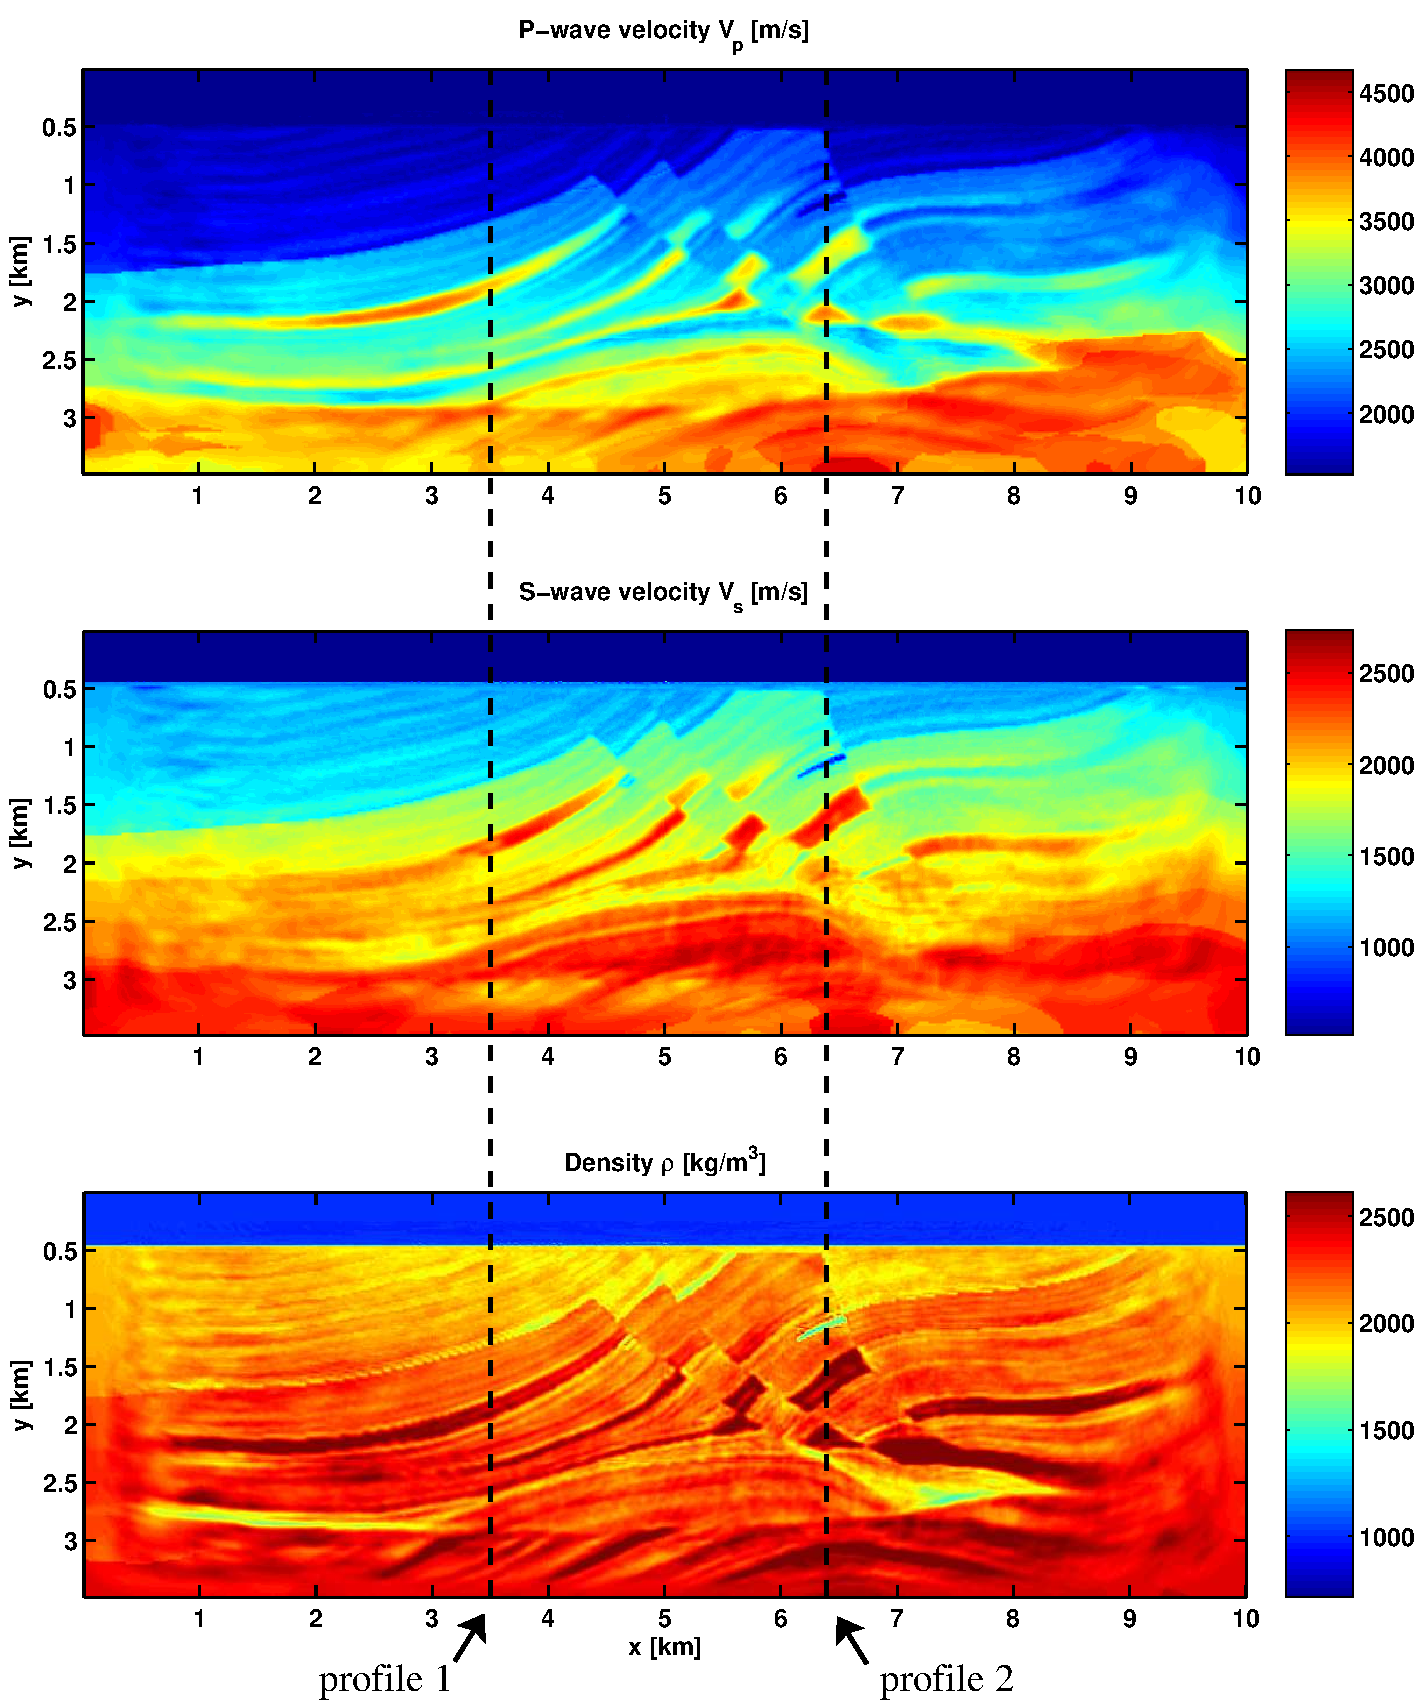
\includegraphics[width=15cm]{figures/marmousi/marmousi_II_result_1.pdf}
\caption{Results of the elastic FWT for the Marmousi-II model. The dashed lines denote the positions of the depth profiles 1 and 2 shown in Fig. \ref{marmousi_II_result_profile}.}
\label{marmousi_II_result}
\end{figure}
\clearpage
It is quite surprising, that the shear wave velocity model could also be resolved very well, even though only streamer data and therefore mainly P-wave information is used. Even the density, a parameter which can be hardly estimated from seismic data, could be recovered from the seismic wavefield. Keep in mind though, that the density image is based not only density information, but contains also $\rm{V_p}$ and $\rm{V_s}$ information due to the ambiguity investigated by the CTS test problem \citep[chapter 5.2]{koehn:11}. The depth profiles show the strong deviation of the starting model from the true Marmousi model, in some parts up to $\rm{\pm 500-1000\;m/s}$ for the velocity models and $\rm{\pm 250-500\;kg/m^3}$ for the density models. Even though the FWT could reconstruct the velocity and density structures quantitatively fairly well. In Fig. \ref{marmousi_seis} the seismic section of shot 50 is plotted for the starting model (a), the inversion result (b) the true model (c), the initial residuals (d), the final residuals (e) and the evolution of the residual energy (f). Notice the good fit of the first arrivals for the starting model, but the lack of small details beyond the first arrivals. Only the direct wave, the reflection from the ocean bottom and a few multiples are present. The inversion result fits most of the phases and amplitudes of the later small scale reflections from within the thrust fault system and therefore the data residuals are very small. The misfit function decreases smoothly for the first 20 Iteration steps, but exhibits strong fluctuations for the later iterations, due to the strong nonlinear character of the inversion problem for this complex geology.  
The performance of the FWT code was benchmarked on an Altix 4700 using the Marmousi2 model. Fig.\ref{bench_time} shows the computation time (top) and the memory requirements for up to 50 CPUs (bottom). On a single CPU the elastic timedomain FWT is not efficient at the moment. For 150 iteration steps a total calculation time of 85 days and about 10 GB of RAM would be required. When using 50 CPUs the computation 
time is reduced to roughly 2 days. Note the linear speedup of the FWT code due to the optimized parallelization of the forward modelling FD code.\\ 
In conclusion the results look very impressive, but you should not forget that the starting model for the seismic velocities and density are unrealistically accurate and are not easy to derive from the seismic data for such a complex model. 
\begin{figure}
\centering
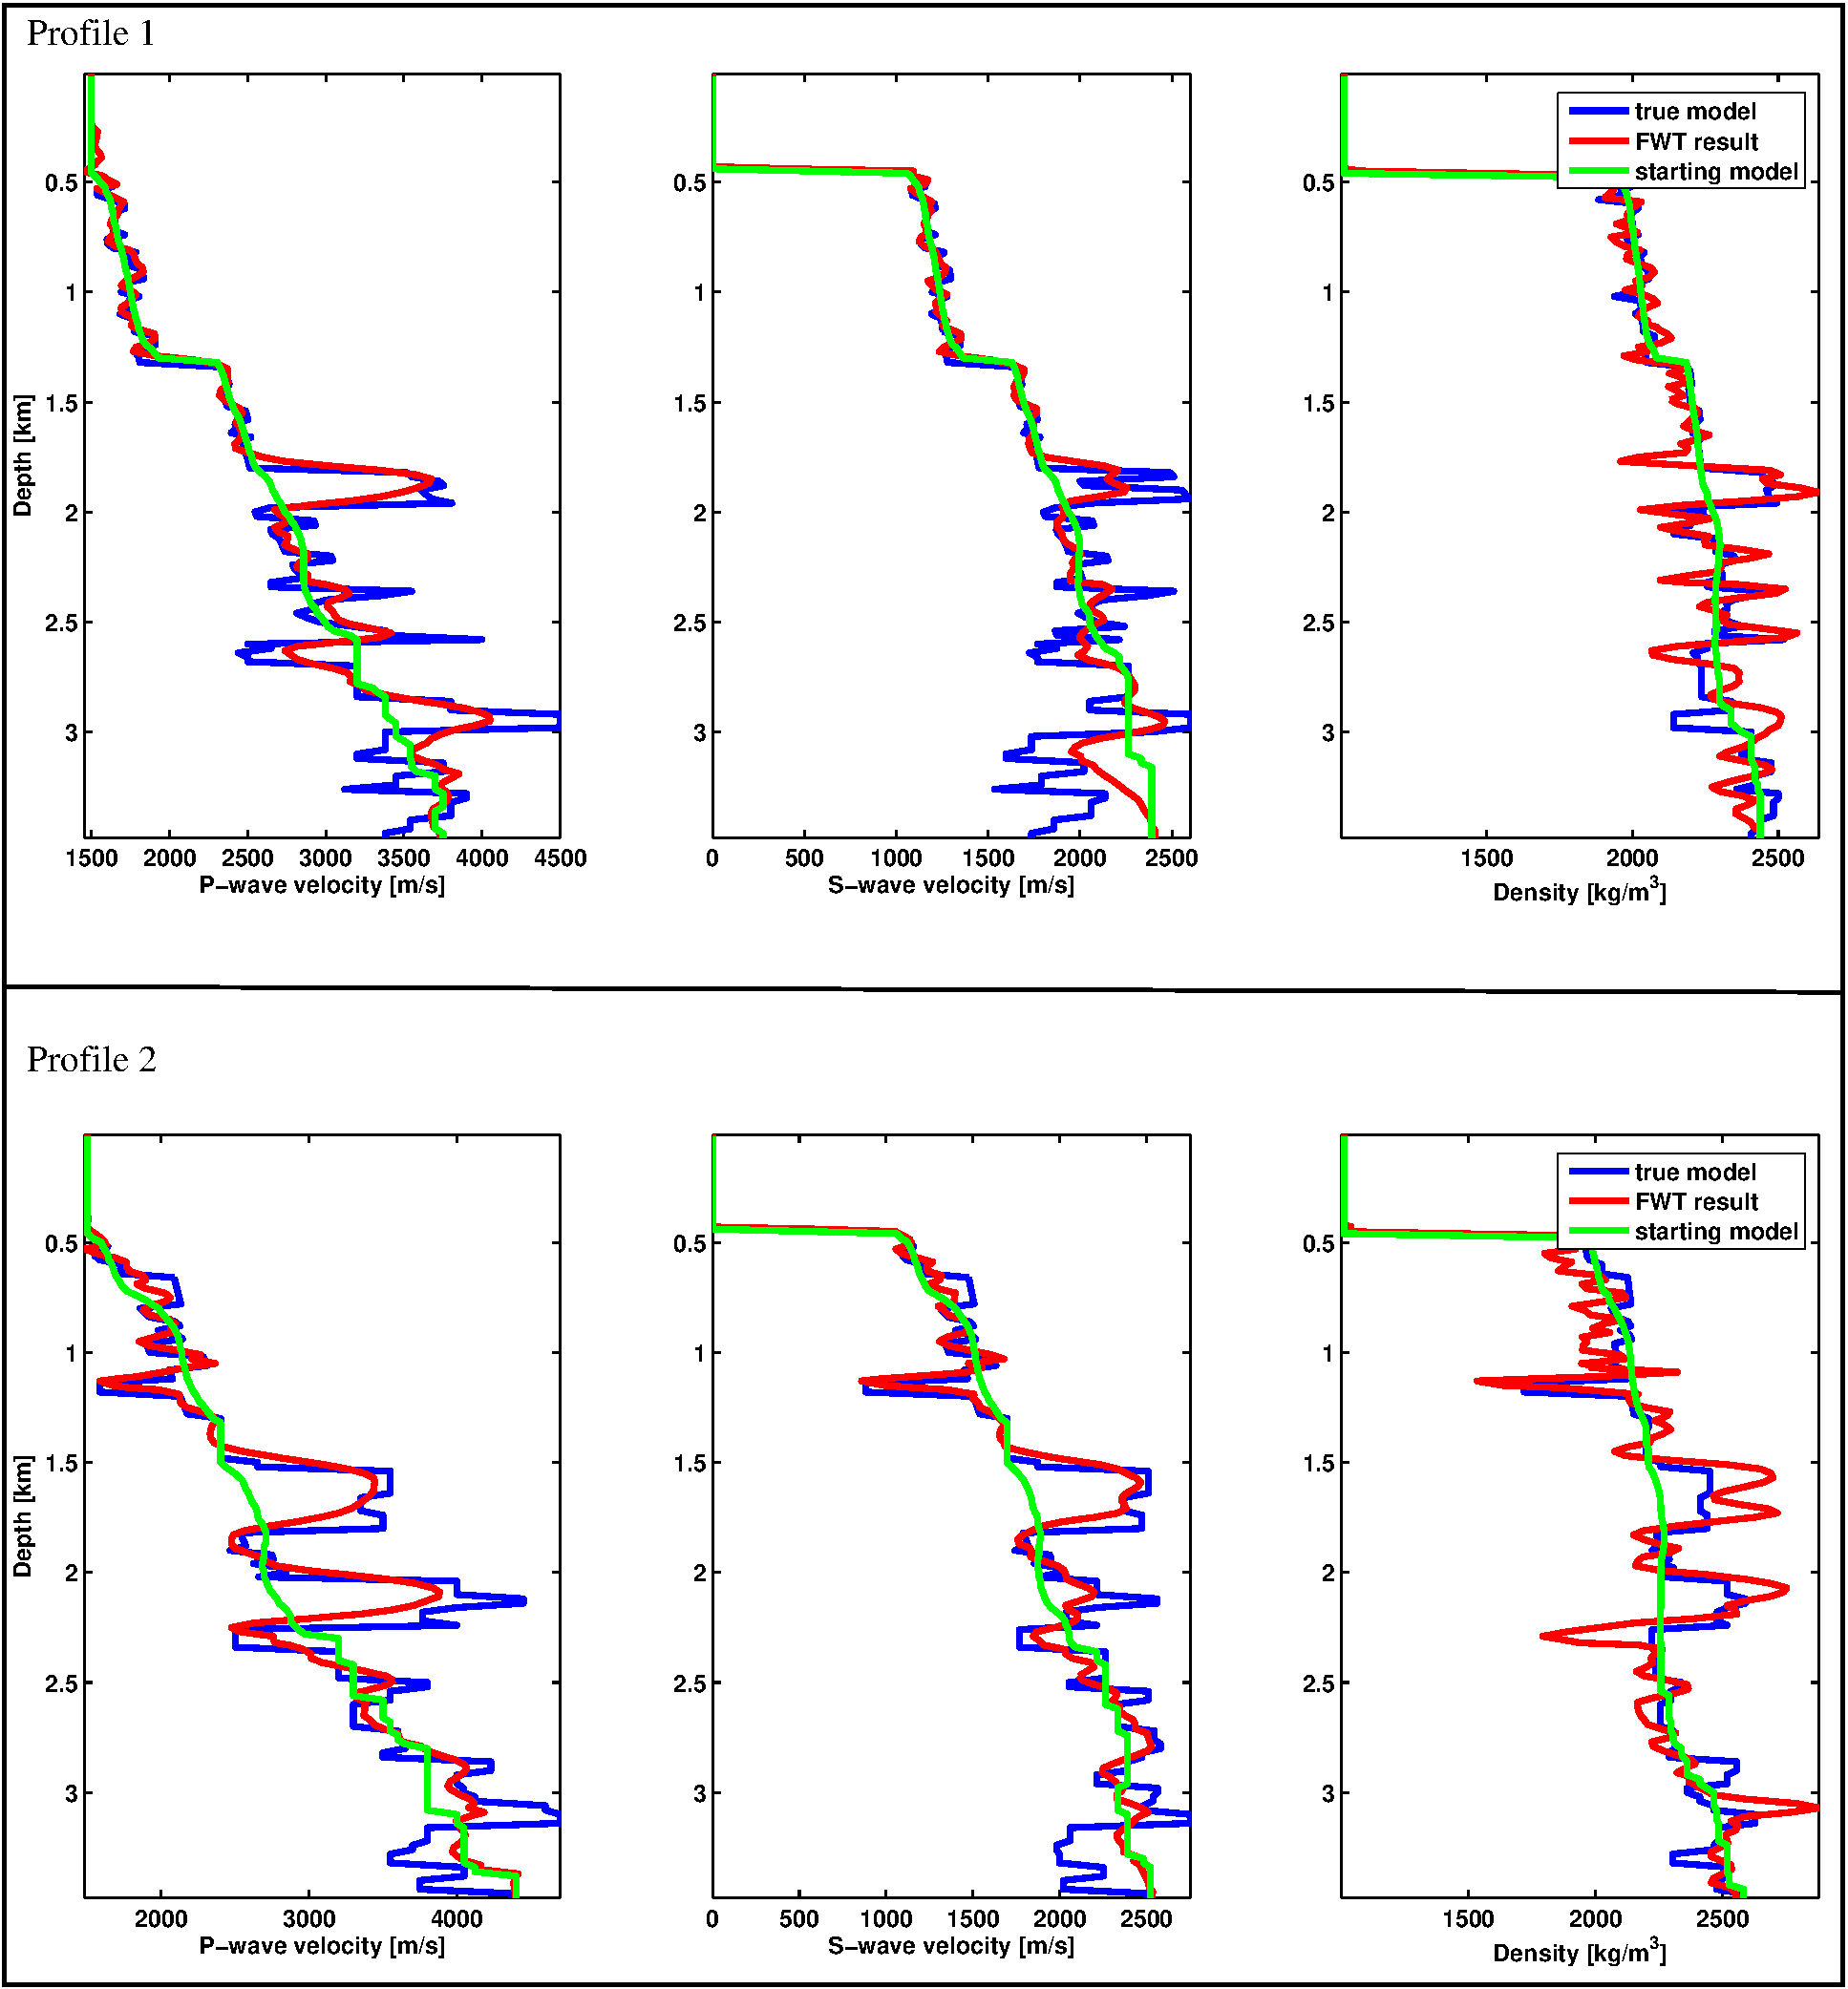
\includegraphics[width=16cm]{figures/marmousi/marmousi_II_result_profile_1.pdf}
\caption{Depth profiles at $\rm{x_{p1}=3.5\;km}$ (top) and $\rm{x_{p2}=6.4\;km}$ (bottom) of the starting model and FWT result are compared with the true model for the Marmousi-II model: P-wave velocity (left), S-wave velocity (center) and density (right).}
\label{marmousi_II_result_profile}
\end{figure}
\clearpage
\begin{figure}
\centering
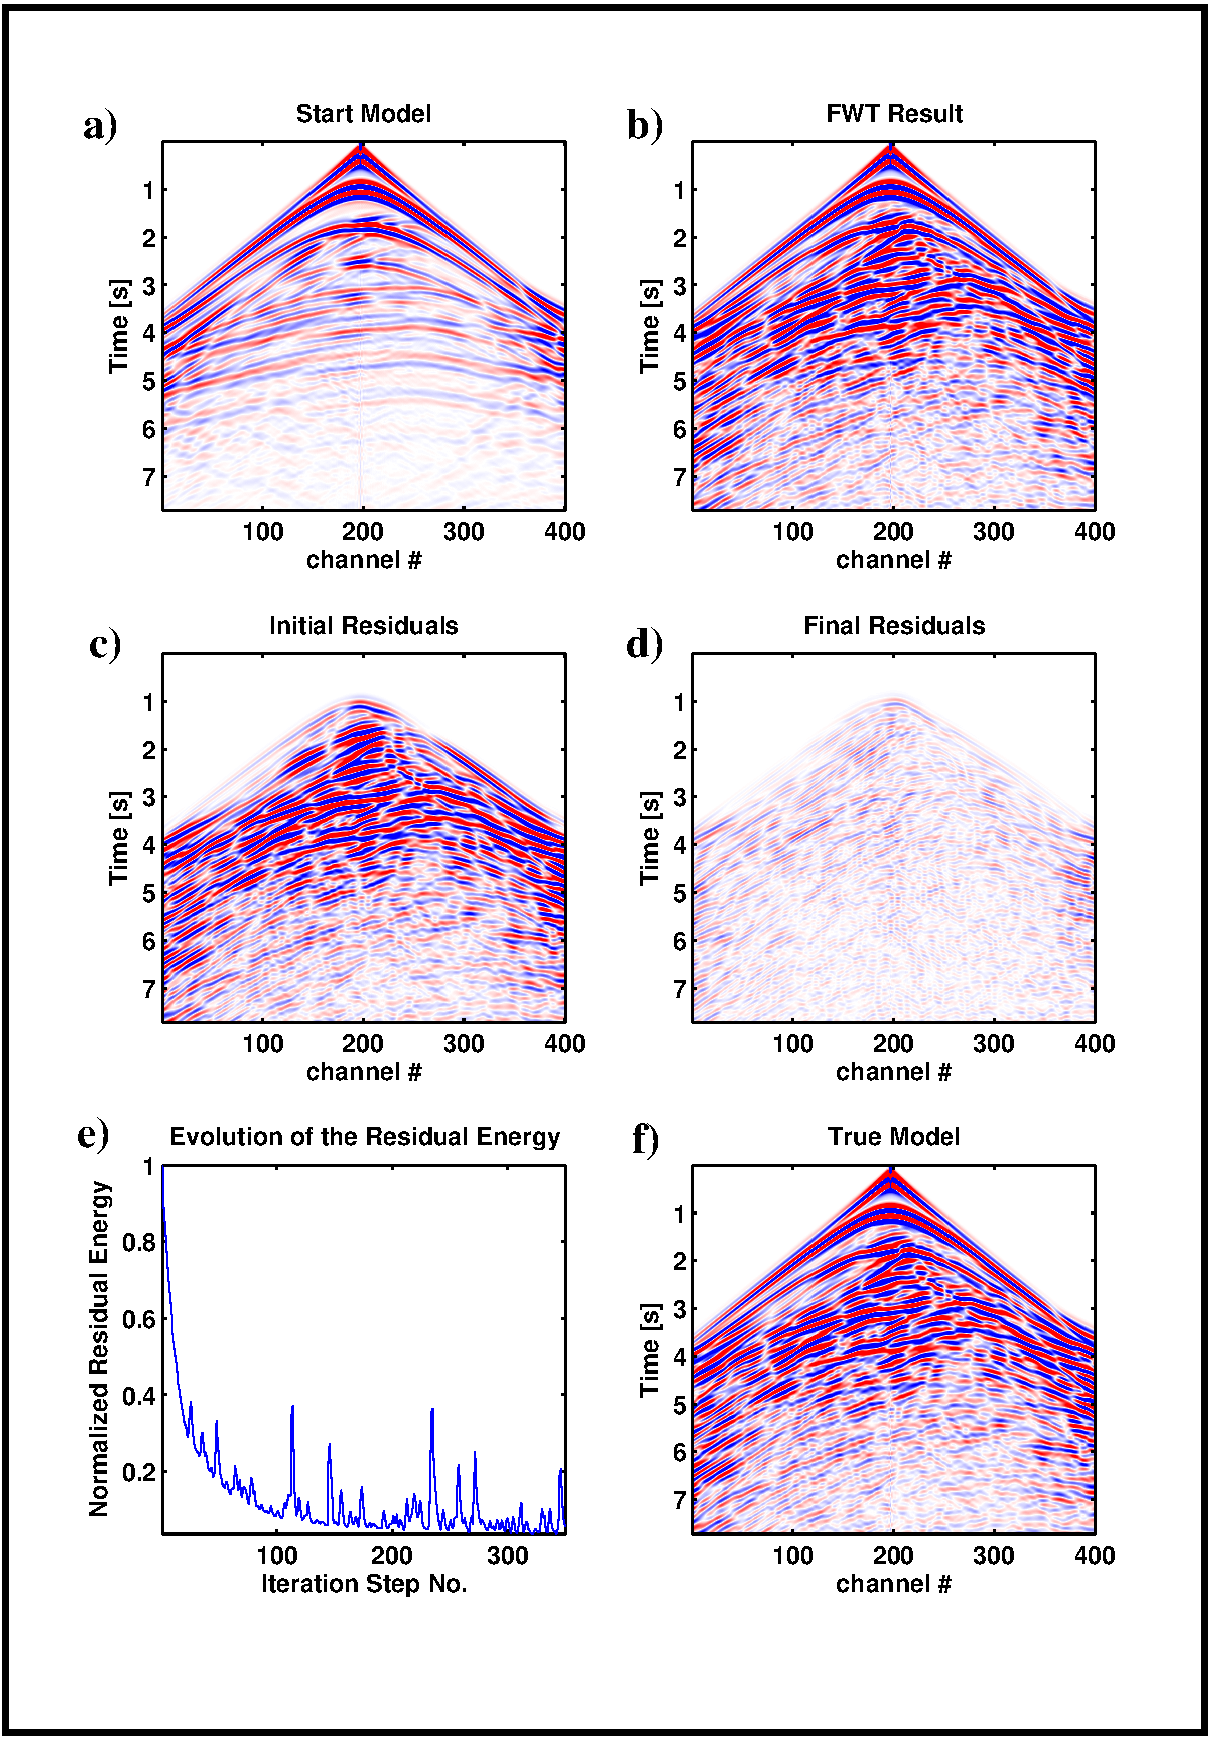
\includegraphics[width=12.5 cm]{figures/marmousi/marmousi_seis_results_WIT.pdf}
\caption{Seismic sections (shot 50, y-component) for the Marmousi-II model. (a) starting model, (b) FWT result, (c) initial residuals, (d) final residuals , (f) true model and (e) evolution of the residual energy.}
\label{marmousi_seis}
\end{figure}
\clearpage
\begin{figure}
\centering
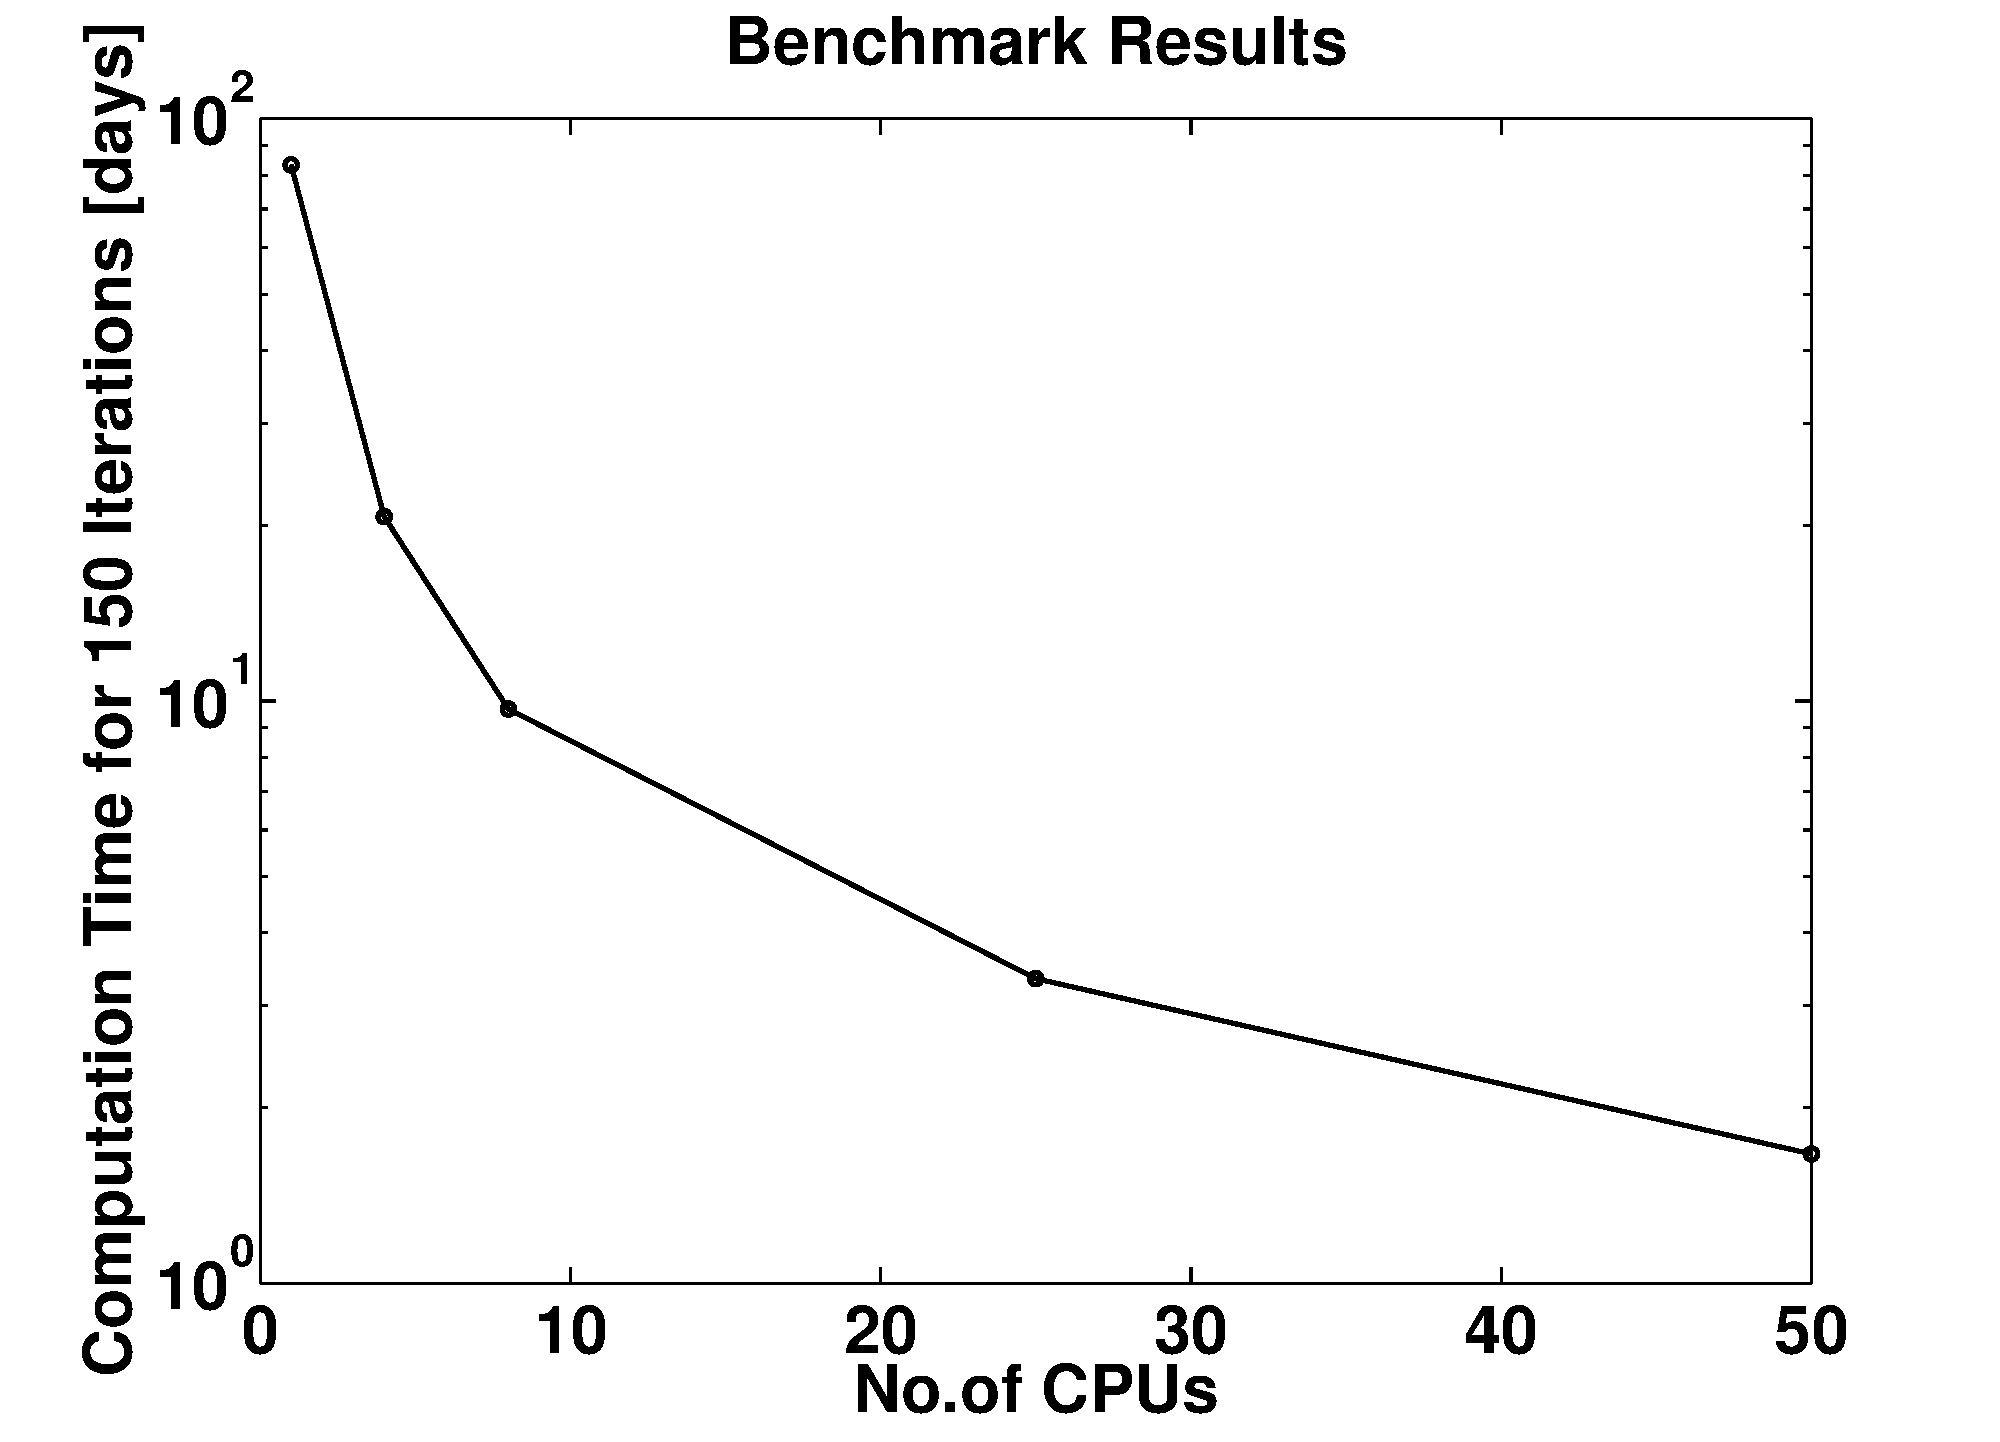
\includegraphics[width=11cm]{figures/marmousi/cpu_altix_DENISE.pdf}\\
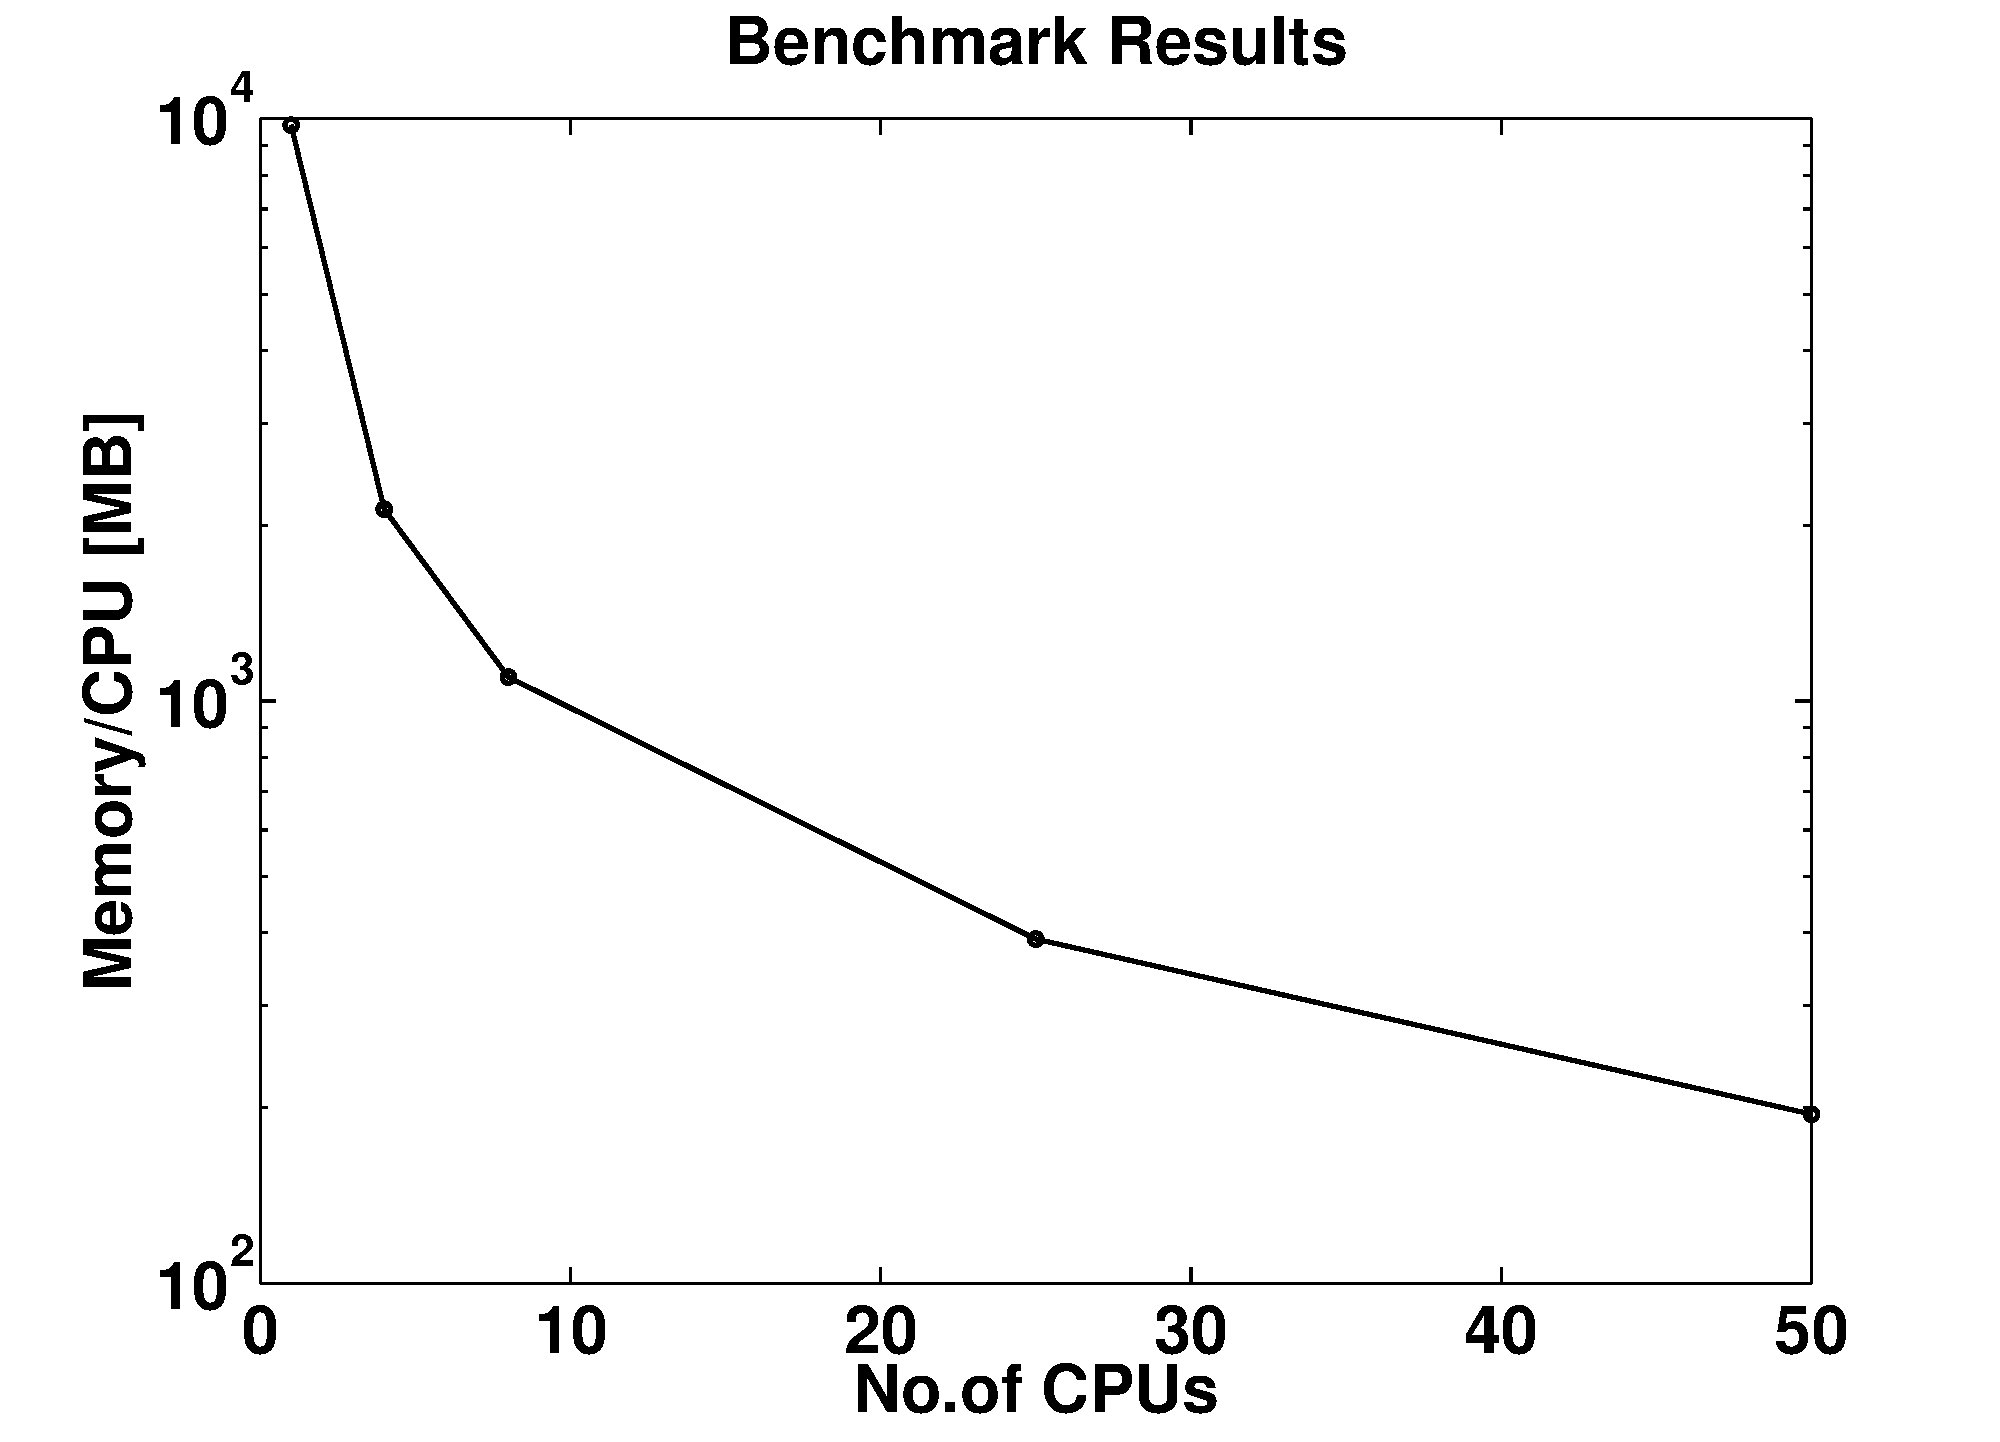
\includegraphics[width=11cm]{figures/marmousi/mem_altix_DENISE.pdf}
\caption{Benchmark results for the Marmousi2 model. The absolute calculation times (top) and the memory requirements (bottom) for up to 50 CPUs on an Altix 4700.}
\label{bench_time}
\end{figure}
\clearpage